%\documentclass[9pt,twocolumn]{scrartcl}


\documentclass[9pt]{sigcomm-alternate}

%\usepackage[margin=1in,bottom=1.2in]{geometry}
\usepackage{amsfonts,amssymb,amsmath}
%\usepackage[thmmarks,hyperref,amsthm,amsmath]{ntheorem}
\usepackage{graphicx}
\usepackage[ruled,vlined,commentsnumbered]{algorithm2e}
\usepackage[usenames,dvipsnames]{color}
\usepackage{hyperref}
\usepackage{multirow}
\usepackage{lineno}
\usepackage[shortlabels]{enumitem}
\usepackage[utf8]{inputenc}
\usepackage[OT4]{fontenc}
\usepackage{comment}
\usepackage{fancyhdr}
\usepackage{tikz}
\usepackage{wrapfig}
%Used Symbols
%c_i = chunk i
%v_i = vm i
%b_t = transfer bandwidth
%b_c = pairwise communication bandwidth
%n = |VMs| = |Chunks|


%Header Extensions Seperation
%Carlo
\newcommand{\VmSlot}{\text{VM slot}}
\newcommand{\VmSlots}{\VmSlot\text{s}}
%\newcommand{\Capacity}{\ensuremath{\textsc{cap}}}
\newcommand{\VM}{\textsc{VM}}
\newcommand{\Problem}{\textsc{DummyName Problem}}
\newcommand{\carlo}[1]{\textcolor{red}{carlo: #1}}
\newcommand{\maciek}[1]{\textcolor{brown}{maciek: #1}}
\newcommand{\stefan}[1]{\textcolor{blue}{stefan: #1}}
\newcommand{\MaFactor}{m}
\newcommand{\Path}{\ensuremath{p}}
\newcommand{\RedundancyFactor}{\ensuremath{r}}

\newcommand{\variab}{\nu}

\newcommand{\Source}{\ensuremath{s^{+}}}
\newcommand{\Sink}{\ensuremath{s^{-}}}

\newcommand{\VmChunkAssignment}{\mu}
\newcommand{\NodeMapping}{\pi}
\newcommand{\ChunkLocation}{\pi}

\newcommand{\ChunkType}{\tau}
\newcommand{\VirtualNodes}{\ensuremath{V}}
\newcommand{\VirtualEdges}{\ensuremath{E_V}}
\newcommand{\VirtualNode}{v}
\newcommand{\VirtualEdge}{e}
\newcommand{\VCSwitch}{\ensuremath{\textsc{center}}}
\newcommand{\SubstrateNodes}{\ensuremath{V_S}}
\newcommand{\SubstrateEdges}{\ensuremath{E_S}}
\newcommand{\SubstrateNode}{\ensuremath{v}}
\newcommand{\SubstrateEdge}{\ensuremath{e}}
\newcommand{\Leaf}{\ensuremath{l}}
\newcommand{\Leaves}{\ensuremath{L}}
\newcommand{\Chunks}{\ensuremath{\textsc{chunks}}}
\newcommand{\aroot}{\emph{root}}

\newcommand{\Opt}{\ensuremath{Opt}}
\newcommand{\Children}{\ensuremath{children}}
%\newcommand{\Cost}{\ensuremath{\textsc{cost}}}

\newcommand{\Uplink}{\ensuremath{\textsc{uplink}}}
\newcommand{\ChunkCount}{\ensuremath{\textsc{cis}}}
\newcommand{\VmCount}{\ensuremath{\textsc{vis}}}
\newcommand{\Right}{\ensuremath{r}}
\newcommand{\InverseAssignment}{\ensuremath{\VmChunkAssignment^{-1}}}

\newcommand{\clauses}{\alpha}
\newcommand{\vars}{\beta}
\newcommand{\variables}{\beta}
\newcommand{\achunk}{\ensuremath{c}}
\newcommand{\Chunk}{\ensuremath{c}}
\newcommand{\capa}{\emph{cap}}
\newcommand{\capacity}{\emph{cap}}
\newcommand{\Distance}{\emph{\textsc{dist}}}
\newcommand{\dist}{\emph{dist}}
\newcommand{\CostPerChunk}{\emph{cost}}


\newcommand{\VC}{\textsc{VC}}
\newcommand{\CC}{\textsc{NI}}

\newcommand{\VE}{\textsc{VE}}
\newcommand{\FP}{\textsc{FP}}
\newcommand{\RS}{\textsc{RS}}
\newcommand{\BW}{\textsc{BW}}
\newcommand{\MA}{\textsc{MA}}
\newcommand{\Cost}{\textsc{F}}

\newcommand{\MatchCost}{\textsc{MCost}}
\newcommand{\chunkOf}{\textsc{chunkOf}}



\newtheorem{defn}{Definition}
\newtheorem{obs}{Observation}

%Maciek

\newcommand{\Bandwidth}{\ensuremath{bw}}
\newcommand{\Tree}{\ensuremath{T}}
\newcommand{\CostTrans}{\ensuremath{b_1}}
\newcommand{\CostCom}{\ensuremath{b_2}}
\newcommand{\Vms}{\ensuremath{n_V}}
\newcommand{\TSC}{\textsc{3-SC}}
\newcommand{\TDM}{\textsc{3-DM}}
\newcommand{\TSAT}{\textsc{3-Sat}}
\newcommand{\NSAT}{\textsc{Sat}}
\newcommand{\SAT}{\textsc{Sat}}
\newcommand{\ZSAT}{\textsc{2-Sat}}


\newcommand{\Formula}{\ensuremath{\Psi}}
\newcommand{\Clauses}{\ensuremath{Cl(\Formula)}}
\newcommand{\NClauses}{\ensuremath{c}}
\newcommand{\Vars}{\ensuremath{Var(\Formula)}}
\newcommand{\NVars}{\ensuremath{|\Vars|}}
\newcommand{\ChunkTypes}{\ensuremath{ch}}
\newcommand{\Thr}{\ensuremath{Th}}
\newcommand{\VCB}{\ensuremath{VCB}}
\newcommand{\VCNB}{\ensuremath{VCNB}}
\newcommand{\varx}{\ensuremath{x}}
\newcommand{\positive}{\ensuremath{positive}}
\newcommand{\negative}{\ensuremath{negative}}
\newcommand{\Val}{\ensuremath{Val}}
\newcommand{\Sol}{\ensuremath{SOL}}



\definecolor{blueLink}{rgb}{0,0.2,0.8}
\hypersetup{colorlinks,linkcolor=blueLink,urlcolor=blueLink,citecolor=blueLink}
\newcommand{\lref}[2][]{\hyperref[#2]{#1~\ref*{#2}}}



%%%%%%%%%%%%%%%%%%%%%%%%%%%%%%%%%%%%%%%%%%%%%%%%%%%%%%%%%%%%%
% GENERAL STYLE MACROS
%%%%%%%%%%%%%%%%%%%%%%%%%%%%%%%%%%%%%%%%%%%%%%%%%%%%%%%%%%%%%

\newcommand{\etal}{{\it et~al.\ }}
\newcommand{\myparagraph}[1]{{\smallskip\noindent{\bf #1}}}
\newcommand{\mycase}[1]{{\underline{Case~#1}:}}

%%%%%%%%%%%%%%%%%%%%%%%%%%%%%%%%%%%%%%%%%%%%%%%%%%%%%%%%%%%%
% THEOREMS AND SUCH
%%%%%%%%%%%%%%%%%%%%%%%%%%%%%%%%%%%%%%%%%%%%%%%%%%%%%%%%%%%%%

\newtheorem{theorem}{Theorem}
\newtheorem{corollary}[theorem]{Corollary}
\newtheorem{lemma}[theorem]{Lemma}
\newtheorem{claim}[theorem]{Claim}
\newtheorem{fact}{Fact}

%%%%%%%%%%%%%%%%%%%%%%%%%%%%%%%%%%%%%%%%%%%%%%%%%%%%%%%%%%%%%
% USEFUL LETTERS
%%%%%%%%%%%%%%%%%%%%%%%%%%%%%%%%%%%%%%%%%%%%%%%%%%%%%%%%%%%%%

\DeclareMathOperator{\polylog}{polylog}
\newcommand{\emdash}{\hspace{1mm}---\hspace{1mm}}
\newcommand{\e}{\mathrm{e}}
\renewcommand{\O}{\mathcal{O}}
\renewcommand{\Pr}{\mathbf{Pr}}
\newcommand{\E}{\mathbf{E}}
\newcommand{\NAT}{\mathbb{N}}
\newcommand{\REAL}{\mathbb{R}}

%%%%%%%%%%%%%%%%%%%%%%%%%%%%%%%%%%%%%%%%%%%%%%%%%%%%%%%%%%%%%
% PARENTHESES ETC
%%%%%%%%%%%%%%%%%%%%%%%%%%%%%%%%%%%%%%%%%%%%%%%%%%%%%%%%%%%%%

\newcommand{\ceiling}[1]{\left\lceil #1 \right\rceil}
\newcommand{\floor}[1]{\left\lfloor #1 \right\rfloor}
\newcommand{\braced}[1]{{\left\{#1\right\}}}
\newcommand{\bigbrackd}[1]{{\big[#1\big]}}
\newcommand{\brackd}[1]{{\left[#1\right]}}
\newcommand{\parend}[1]{{\left(#1\right)}}

%%%%%%%%%%%%%%%%%%%%%%%%%%%%%%%%%%%%%%%%%%%%%%%%%%%%%%%%%%%%%
% FRACTIONS
%%%%%%%%%%%%%%%%%%%%%%%%%%%%%%%%%%%%%%%%%%%%%%%%%%%%%%%%%%%%%

\newcommand{\half}{\frac{1}{2}}
\newcommand{\onehalf}{\frac{1}{2}}
\newcommand{\onethird}{\frac{1}{3}}
\newcommand{\twothirds}{{\textstyle\frac{2}{3}}}
\newcommand{\fourthirds}{{\textstyle\frac{4}{3}}}
\newcommand{\fivethirds}{{\textstyle\frac{5}{3}}}
\newcommand{\threefourths}{{\textstyle\frac{3}{4}}}

%%%%%%%%%%%%%%%%%%%%%%%%%%%%%%%%%%%%%%%%%%%%%%%%%%%%%%%%%%%%%
% ALGORITHM NAMES, ETC
%%%%%%%%%%%%%%%%%%%%%%%%%%%%%%%%%%%%%%%%%%%%%%%%%%%%%%%%%%%%%

\newcommand{\ALG}{\textsc{Alg}}
\newcommand{\OPT}{\textsc{Opt}}
\newcommand{\DET}{\textsc{Det}}
\newcommand{\RAND}{\textsc{Rand}}

%%%%%%%%%%%%%%%%%%%%%%%%%%%%%%%%%%%%%%%%%%%%%%%%%%%%%%%%%%%%%
% PSEUDOCODE
%%%%%%%%%%%%%%%%%%%%%%%%%%%%%%%%%%%%%%%%%%%%%%%%%%%%%%%%%%%%%

\newcommand{\IF}    {{\bf if }}
\newcommand{\THEN}  {{\bf then }} 
\newcommand{\FOR}   {{\bf for }}
\newcommand{\EACH}  {{\bf each }} 
\newcommand{\DO}  {{\bf do }} 

%%%%%%%%%%%%%%%%%%%%%%%%%%%%%%%%%%%%%%%%%%%%%%%%%%%%%%%%%%%%%
% EDITORIAL MACROS
%%%%%%%%%%%%%%%%%%%%%%%%%%%%%%%%%%%%%%%%%%%%%%%%%%%%%%%%%%%%%

\definecolor{brown}{rgb}{0.4,0,0} 
\definecolor{purple}{rgb}{0.2,0,0.6}
\definecolor{hotpink}{rgb}{1,0.4,0.7}
\newcommand{\marginnote}[1]{\marginpar{\scriptsize{\begin{flushleft}#1\end{flushleft}}}}
\newcommand{\todo}[1]{\noindent\colorbox{red}{todo: #1}} 
\newcommand{\marcin}[1]{\color{red} Marcin: #1\color{black}}



\title{A Note on Virtual Cluster Embedding with Data Locality}

\title{Embedding Algorithms for Virtual Clusters with Data Locality and Replica Selection}

\title{Embedding Virtual Clusters with Data Locality and Replica Selection\\{\Large Real Algorithms for Virtual Environments}}

\title{Data Locality and Replica Aware Virtual Cluster Embeddings}
%\\{\Large Real Algorithms for Virtual Environments}}


\author{Carlo Fuerst$^1$, Maciej Pacut$^2$, Stefan Schmid$^3$\\
{\small $^1$ TU Berlin, Germany; $^2$ University of Wroclaw, Poland; $^3$ TU Berlin \& T-Labs, Germany}}

\begin{document}

\maketitle


\begin{abstract}
Virtualized datacenters offer great flexibilities in terms of resource allocation. In particular, by
decoupling applications from the constraints of the underlying physical infrastructure, virtualization
supports an optimized mapping of virtual machines as well as their interconnecting network
% (the so-called \emph{virtual cluster})
to their
physical counterparts: essentially a graph embedding problem.

However, existing algorithms
in the literature often ignore a crucial dimension of the embedding problem, namely \emph{data locality}:
the input to a cloud application such as MapReduce is typically stored in a distributed,
and sometimes redundant, file system. Since moving
data is costly, an embedding algorithm should be data locality aware,
and allocate computational resources close to the data; in case of redundant storage, the algorithm should also optimize the \emph{replica selection}.

This paper initiates the algorithmic study of data locality aware virtual cluster embeddings
% for
%the widely used (fat-)tree like
on datacenter topologies.
In particular, we
show that
despite the multiple degrees of freedom in terms of embedding and replica selection,
many problems can be
solved efficiently, and we highlight interesting connections
to classic optimization problems. However, we also show the limitations of such optimizations,
by presenting several new NP-hardness results; interestingly,
our hardness proofs even hold in uncapacitated settings.
\end{abstract}

\begin{comment}
we should maybe give the main algorithms a name; we should talk about the case where the number of machines is not a perfect multiple;
\end{comment}

\section*{TODOs}

determine all runtimes (check related work for flow and match!), make float-figures, finish appendix, order properties in the same way always (the order we had in the model!), make all $O$-notations the same $\mathrm{O}$

%%%%%%%%%%%%%%%%%%%%%%%%%%%%%%%%%%%%%
\section{Introduction}

%Server virtualization has revamped the server business over the last years,
%and has radically changed the way we think about resource allocation:
%today, almost arbitrary computational resources can be allocated on demand.
%Moreover, the virtualization trend now started to spill over to the network:
%batch-processing applications such as MapReduce often generate significant
%network traffic (namely during the so-called shuffle phase)~\cite{amazonbw},
%and in order to avoid interference in the underlying physical network and in order to provide a predictable
%application performance, it is important to provide performance isolation and bandwidth guarantees
%for the virtual network connecting the virtual machines.~\cite{talk-about}

Server and link virtualization introduces interesting resource allocation flexibilities,
in the sense that virtual machines and their interconnecting network,
can in principle be embedded \emph{anywhere} in the datacenter.
The resource allocation flexibilities
can in principle be exploited to improve resource sharing.

A very popular abstraction for batch-processing applications such as MapReduce is the \emph{virtual cluster}~\cite{oktopus}:
As batch-processing applications often generate significant
network traffic (namely during the so-called \emph{shuffle phase})~\cite{amazonbw},
in order to avoid interference in the underlying physical network and in order to ensure a predictable
application performance,
it is important to provide performance isolation and bandwidth guarantees between virtual machines.~\cite{talk-about}
Accordingly, a virtual cluster not only defines a set of virtual machines offering computational resources,
but also an interconnecting network with (symmetric and pair-wise) bandwidth guarantees: essentially a \emph{virtual network}.

Several algorithms have been proposed over the last years to map virtual machines as close as possible
to each other in the datacenter, which minimizes communication costs (i.e., bandwidth reservations).~\cite{oktopus,proteus}
However, existing embedding algorithms ignore the input to the batch-processing applications:
the (input) \emph{data}. Often, data is stored in a distributed file system, on different servers,
and in order to minimize
communication costs, an embedding algorithm should be \emph{data locality aware},
and allocate (or \emph{embed}) computational resources close to the to be processed data. Moreover, in case of redundant storage (batch processing
applications often provide a 3-fold redundancy), the algorithm should also exploit \emph{replica selection}
flexibilities.

\subsection{Our Contributions}

This paper initiates the study of data-locality and replica aware embedding problems in virtualized datacenters.
In particular, we decompose the optimization problem into different fundamental aspects, such as
replica selection and flexible virtual machine embedding, and answer questions such as:
\begin{enumerate}
\item How to efficiently select and assign replicas to virtual machines?

\item How to efficiently embed virtual machines and their inter-connecting network?

\item Can the replica selection and virtual machine embedding be jointly optimized, in polynomial time?
\end{enumerate}

We draw an almost complete picture of the problem space: We show that
even problem variants exhibiting multiple degrees of freedom (in terms of
replica selection and embedding),
can be solved optimally in polynomial time, and compare different
algorithmic approaches; however, we also prove limitations in terms of
computational tractability, by providing reductions from 3-D matching
and Boolean satisfiability ($\SAT$). Interestingly,
while it is well-known that (unsplittable) multi-commodity flow
problems are NP-hard in capacitated networks, our hardness results also hold in \emph{uncapacitated}
networks; moreover, we show that NP-hard problems already arise in small-diameter networks (as they are
widely used today~\cite{fattree}),
and even if the number of replicas is bounded by two.


\subsection{Organization}

The remainder of this paper is organized as follows.
Section~\ref{sec:model} introduces our formal model in detail.
Algorithms are presented in Section~\ref{sec:poly} and
hardness results are presented in Section~\ref{sec:np}.
After discussing related work in Section~\ref{sec:relwork},
we conclude our work in Section~\ref{sec:conclusion}.
Some technical details as well as additional hardness results
appear in the Appendix.

\section{Model}\label{sec:model}

To get started, let us first introduce our model as well as its constituting parts \emph{formally}.
For the sake of clarity, we defer the discussion of the practical background and motivation
to the end of this section. Figure~\ref{fig:overview} gives an overview of our model.

\begin{figure}[t]
\centering
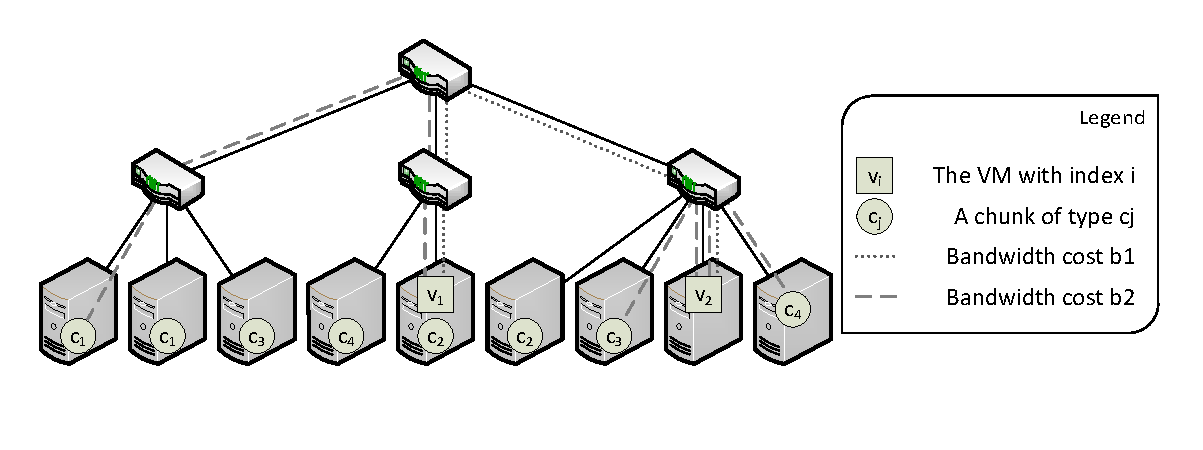
\includegraphics[width=0.99\columnwidth]{figs/overview-fig.pdf}
\caption{Overview: a 9-server (fat-tree) datacenter storing 4 different chunk
types $\{c_1,\ldots,c_4\}$ (depicted as \emph{circles}). The chunk replicas need to be selected and assigned to the two
 virtual machines $v_1$ and $v_2$; the virtual machines are depicted as \emph{squares}, and
 the network connecting them to chunks is \emph{dashed}. In addition, the virtual machines are inter-connected among
 each other (\emph{dotted}). The objective of the embedding problem is to minimize the overall bandwidth allocation
 (sum of dashed and dotted lines).}
\label{fig:overview}
\end{figure}


%\textbf{Fundamental Parts.}

\subsection{Fundamental Parts}

Our model consists of three fundamental parts: (1) the substrate network (the servers
and the connecting physical network),
(2) the to be processed input (the data), and
(3) the virtual network (the virtual machines and the logical network connecting the machines to each other
as well as to the data).

\emph{The Substrate Network.} The substrate network (also known as the \emph{host graph}) represents the physical resources:
a set $S$ of $n_S=|S|$ servers interconnected by a network consisting of a set $R$ of servers (or switches)
and a set $E$ of (symmetric) links. (We will sometimes simply refer to the elements in $S$ and $R$
as the \emph{vertices}.) We will assume that the inter-connecting network forms an (arbitrary, not necessarily balanced
or regular) tree,
where the servers are located at the tree leaves.
Each server $s\in S$ can host a certain number
of virtual machines (available server capacity $\capacity(s)$), and each link $e\in E$ has a certain bandwidth
capacity $\capacity(e)$.

\emph{The Input Data.} The to be processed data constitutes the input to the batch-processing application.
The data is stored in a distributed manner; this spatial distribution is given and not subject to optimization.
The input data consists of different \emph{chunk types} $\{\achunk_1, \ldots, \achunk_{\ChunkType}\}$,
where each chunk type $\achunk_i$ can have $r\geq 1$ instances (or replicas) $\{\achunk_{i}^{(1)},\ldots, \achunk_{i}^{(r)}\}$,
 stored at different servers. (A single server may host multiple chunks.)
%Concretely, for each of the $r\cdot k$ replicas $\achunk_{i}^{(j)}$.
%, we will denote by $\pi(\achunk_{i}^{(j)})$ at
%which server it is stored \maciek{Do we use $\pi$ anywhere else in paper?}.
It is sufficient to process one replica, and we will sometimes refer to this
replica as the \emph{active} (or selected) replica.

\emph{The Virtual Network.} The virtual network consists of a set $\VirtualNodes$ of $n_V=|\VirtualNodes|$ virtual machines or compute
 units, henceforth often simply called \emph{nodes}.
Each node $v \in \VirtualNodes$ can be placed (or, synonymously, \emph{embedded}) on a server; this placement can be subject
to optimization.
Depending on the available capacity $\capacity(s)$ of server $s$, multiple nodes maybe be hosted on $s$.
We will denote the server $s$ hosting node $v$ by $\pi(v)=s$.
Since these virtual machines process the input data, they need to be assigned and connected to the
chunks. Concretely, for each chunk type $\achunk_i$, one replica $\achunk_{i}^{(j)}$ must be processed by exactly one virtual machine $v$;
which replica $\achunk_{i}^{(k)}$ is chosen is subject to optimization.
We will denote by $\mu$ the assignment or ``matching'' of virtual
machines to chunks \maciek{matching is an assignment}.
We will keep the model general, and consider both the case where there are more chunk types
than virtual machines (requiring the assignment of multiple chunks per nodes) and the case
where there are less chunks than virtual machines. (See below for motivations for the different scenarios.)
However, in order to avoid stragglers, we require that each node needs to process the same number of chunks;
we will refer to the average number of chunks per node by $\MaFactor$.
Moreover, in order to ensure a predictable performance, both the connection to the chunks
as well as the interconnection between the virtual machines may have to ensure certain
minimal bandwidth guarantees; we will refer to the first type of virtual network as the \emph{(chunk) access
network}, and to the second type of virtual network as the \emph{(shuffle) inter-connect}. The inter-connect
is modeled as a complete network. Concretely, we assume that an  active chunk
is connected to its node at a minimal bandwidth $\CostTrans$, and a node is connected to any other node
at minimal bandwidth $\CostCom$.

%\stefan{TODO: clarify whether there can be multiple chunks and or nodes per server}

%\textbf{Optimization Objective.}

\subsection{Optimization Objective}

Our goal is to develop algorithms which minimize
the \emph{resource footprint}: the overall bandwidth allocation for a given embedding. (Note that
only the resource allocation at the links but not at the servers depends on the replica selection or embedding.) That is,
we aim to embed the virtual machines in a locality-aware manner, close to the input data
(the chunks), as well as close to
each other. Let $\dist(v,\achunk)$ denote the distance (in the underlying physical network $\Tree$) between a node $v$ and
its assigned (active) chunk replica $\achunk$, and let $\dist(v_1,v_2)$ denote the distance between the two nodes $v_1$ and $v_2$.
We define the \emph{footprint} $\Cost(v)$ of a node $v$ as follows:
$$
\Cost(v) = \sum_{\achunk\in \mu(v)} \CostTrans \cdot \dist(v,\achunk) \underbrace{+ \sum_{v' \in \VirtualNodes\setminus\{v\}} \CostCom \cdot \dist(v,v')}_{\text{only for inter-connect}},
$$
\noindent where $\mu(v)$ is the set of chunks assigned to $v$. Our goal is to minimize the overall footprint
$\Cost=\sum_{v\in V} \Cost(v)$.

%\textbf{Problem Decomposition.}

\subsection{Problem Decomposition}

In order to chart the landscape of the tractability and intractability of different
problem variants, we decompose our problem into its fundamental parts, as described in the following.

\emph{Replica Selection ($\RS$).} The first fundamental problem is replica selection:
if the input data is stored redundantly, the algorithm has the freedom to choose a replica
for each chunk type, and assign it to a virtual machine (i.e., \emph{node}). Note that this
selection or ``matching problem'' is non-trivial, even if the locations of the virtual machines
are already given \maciek{it is trivial in locations are not given}. In the following, we will refer to a scenario
with redundant chunks by $\RS$; in the $\RS$-only scenario, the number of chunk types
is equal to the number of nodes. Otherwise, we will add the $+\MA$ property discussed next.

\emph{Multiple Assignment ($\MA$).}
If the number of chunk types is larger than the number of virtual machines,
each node needs to be assigned multiple chunks. We will refer to such a scenario by $\MA$.
(Note that in a scenario with only $\MA$ but without $\RS$, chunk types are not redundant.)

\emph{Flexible Placement ($\FP$).} The second fundamental degree of freedom, besides replica selection and assignment,
regards the flexibility in the placement (or synonymously: \emph{embedding}) of virtual machines to physical servers.
We will refer to this aspect by $\FP$. (Recall that each server $s$ can host $\capa(s)$ nodes.)

%\maciek{Here we would like to
%  introduce hosting multiple VMs in one leaf. How do we do that - by
%  setting global upper bound on number of VMs per leaf - or by
%  per-leaf constant? We also need to update NP-hardness proofs to set
%  those numbers to 1 and to modify the dynamic program's base case.}

\emph{Node Interconnect ($\CC$).} We will distinguish between scenarios where bandwidth needs to be reserved
both from each virtual machine to its assigned replicas as well as to the other virtual machines
(i.e., $\CostTrans>0$ and $\CostCom>0$), and
 scenarios where only the access network requires bandwidth reservation (i.e., $\CostTrans>0$ and $\CostCom=0$).
 We will refer to the former scenarios
where bandwidth needs to be reserved also for the inter-connect, by $\CC$.

\emph{Bandwidth Capacities ($\BW$).}
We distinguish between an uncapacitated and a capacitated scenario where the links
of the substrate network come with bandwidth
constraints, and will refer to the bandwidth-constrained version by $\BW$; the capacity of servers
(the number of virtual machines which can be hosted concurrently) is always limited.
Note that capacity constraints introduce infeasible problem instances, where it is impossible to
allocate sufficient resources to satisfy an embedding request.
%; in this case, we will say that the
%resource footprint is \emph{infinite}. \maciek{I do not like defining
%  value of footprint of infeasible instance. What is the motivation
%  for that?}

%\textbf{Remark on Practical Motivation.}

\subsection{Practical Motivation}\label{ssec:practice}

We conclude our model discussion by providing the necessary practical background and motivation.
Our model is motivated by batch-processing applications such as MapReduce.
Such applications use multiple compute units or virtual machines to
process data, initially often redundantly stored in a distributed file system implemented
by multiple servers.~\cite{mapreduce}
The standard datacenter topologies today are (multi-rooted) fat-tree resp.~\emph{Clos} topologies,~\cite{vl2,fattree}
hierarchical networks  recursively made of sub-trees at each level; this motivates our
focus on tree-like substrate networks where servers are located at the
tree leaves. In particular, given the amount of multiplexing over the mesh of links
and the availability of multi-path routing protocol, e.g.~ECMP, the redundant
links can be considered as a single aggregate link for bandwidth
reservations. This is consistent with similar assumptions made in
previous work~\cite{oktopus,proteus}.

During execution, batch-processing applications typically cycle through different phases,
most prominently, a mapping phase and a reducing phase; between the two phases,
a shuffling operation is performed, a phase where the results from the mappers
are communicated to the reducers. Since the shuffling phase can constitute a
non-negligible part of the overall runtime~\cite{orchestra},
and since concurrent network transmissions can introduce interference and
performance unpredictability~\cite{amazonbw}, it is important
to provide explicit minimal bandwidth guarantees.~\cite{talk-about}
In particular, our inter-connect (the virtual network connecting the virtual machines)
is motivated by the popular virtual cluster abstraction.~\cite{oktopus,talk-about,proteus}
In this paper, we extend this model with a notion of data-locality.
In particular, we distinguish between the bandwidth needed between replica
and virtual machine ($\CostTrans$) and the bandwidth needed between
two virtual machines ($\CostCom$); in practice, for applications with a large
``mapping ratio'' where the mapping phase already reduces the data size significantly,
$\CostCom<\CostTrans$. Finally, note that it is frequently assumed
that the nodes implementing the mapper functionality also implement the reducer functionality,
and vice versa; however, it can also make sense to have more mappers or more reducers for
certain applications.

%%%%%%%%%%%%%%%%%%%%%%%%%%%%%%%%%%%%%
\section{Polynomial-Time Algorithms}\label{sec:poly}

Despite the various degrees of freedom in terms of embedding and replica selection,
 many problem variants can be solved efficiently.
 This section introduces three general techniques to solve different problem variants,
 which can roughly be categorized into
 \emph{flow} (Section~\ref{ssec:flow}), \emph{matching} (Section~\ref{ssec:match}) and \emph{dynamic programming}
 (Section~\ref{ssec:dyn}) approaches.
 As we will see, several problems variants can be solved in multiple ways (but at different runtimes),
 and in each approach, we will indicate the solvable problem variants using a \emph{Venn diagram}.

First, let us make a simplifying observation: 
in problems without flexible placement ($\FP$), 
the bandwidth required
for the inter-connect network ($\CC$) can generally be allocated \emph{upfront}, as it
does not depend on the replica
selection and assignment.
Accordingly, problem variants such $\RS+\MA+\CC +\BW$ or
$\RS+\MA+\CC$ can be reduced to $\RS+\MA+\BW$ resp.~$\RS + \MA$. 

\subsection{Flow Algorithms ($\RS+\MA+\CC+\BW$)}\label{ssec:flow}

\begin{wrapfigure}{r}{0.5\columnwidth}
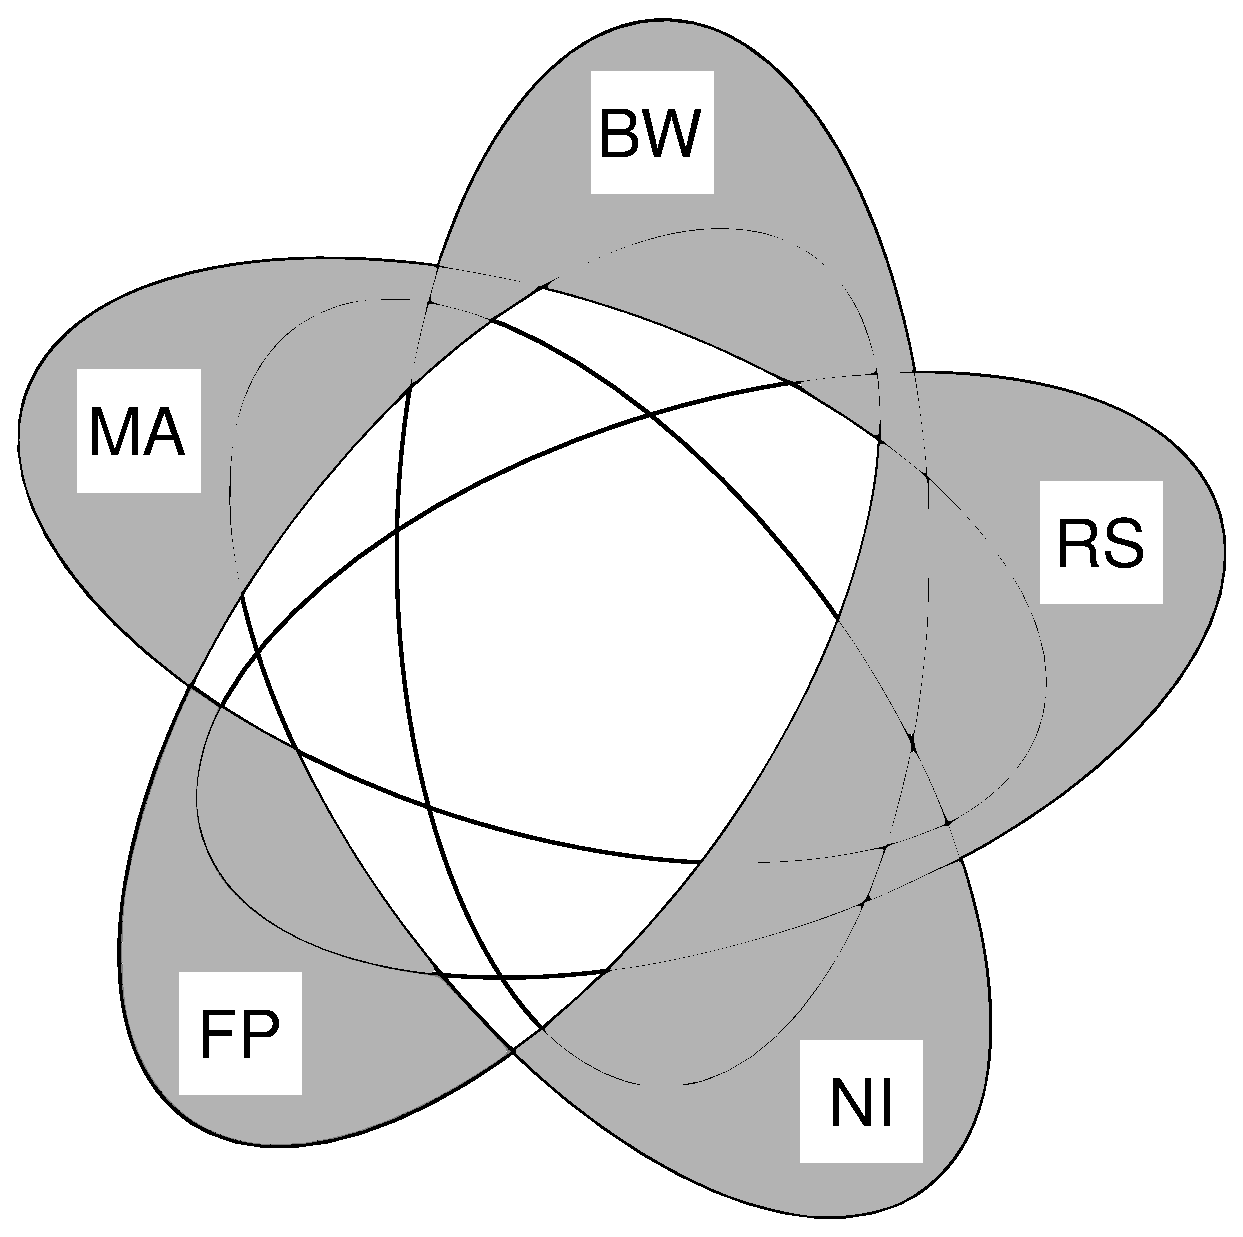
\includegraphics[width=0.48\columnwidth]{figs/venn_flow.pdf}
\caption{Variants solved by flow approach.}
\label{fig:venn_flow}
\end{wrapfigure}

We first present an algorithm to solve the $\RS+\MA+\CC+\BW$ problem.
Recall that in this problem variant,
we are given a set of redundant chunks ($\RS$) and a set of virtual machines
(the \emph{nodes})
at fixed locations (no $\FP$). The number of chunk types is larger than the number
of nodes ($\MA$), and each node needs to be connected
to its selected chunks as well as to other nodes ($\CC$), while respecting
capacity constraints ($\BW$).
Our goal is to minimize the resource footprint $\Cost$, consisting
of the bandwidth reservations in the (chunk) access network and the (node)
inter-connect.
As we will see in the following, a flow algorithm can be used to solve this
problem variant.

%\maciek{We do not need any assumption about bandwidth. If we do not
%  have integrality, we round down every bandwidth. If we do not have
%  multiplicity of $\CostTrans$, we round to highest $\CostTrans \cdot
%  k$. We can deal with mixing $\CostTrans$ and $\CostCom$ by first
%  decreasing bandwidth by (constant) cost of communication, and then
%  rounding down.}

%We allow an instance to have multiple virtual machines in single leaf.

\textbf{Construction of Artificial Graph.}
In order to solve the $\RS+\MA+\CC+\BW$ problem,
we first construct
an artificial graph $\Tree^*$, extending the substrate network $\Tree$ and
normalizing bandwidth capacities, as follows. For $\Tree^*$,
we normalize the bandwidth of $\Tree$ to integer multiples of $\CostTrans$,
i.e., for each link $e\in E(\Tree)$, we set its new
capacity in $\Tree^*$ to $\lfloor\capacity(e)/\CostTrans\rfloor$.
%\maciek{I do not understand the floor here. I strongly suggest setting
%$\CostTrans$ to $1$ in the model}
After this normalization, we extend the $\Tree$ topology by
introducing an artificial vertex for each chunk type. These artificial
vertices are connected to each leaf (i.e., server) in $\Tree$ where replicas of the respective type are located,
connecting the replica of the respective chunk type by a link of capacity $1$. In
addition, we create a
\emph{super-source} $\Source$, and connect it to each of the artificial chunk
type vertices (with a link of capacity 1). Moreover, we create an artificial \emph{super-sink} $\Sink$ and
connect it to every leaf containing at least one node; the link capacity represents 
the number of nodes $x$ hosted on this node, times the multi-assignment factor 
$\MaFactor$: 
$x \cdot \MaFactor$. 
We additionally assign the following costs to edges of $\Tree^*$:
every edge of the original substrate network costs one unit, and all other edges
cost nothing.

Recall that $\RS+\CC+\MA+\BW$ boils down to
$\RS+\MA+\BW$ in the absence of $\FP$
The $\RS+\MA+\BW$ problem can now be solved by computing
a \emph{Min-Cost-Max-Flow} solution between super-source and super-sink on the artificial graph $\Tree^*$.
Figure~\ref{fig:flow_construction} shows an example of the extended substrate
network $\Tree^*$: The source $\Source$ is connected to the two leaves, which host the
virtual machines. The artificial nodes are depicted below the leaves, are labeled with
their respective chunk types (e.g., $\achunk_1$), and are connected to the sink
$\Sink$ as well as to the leaves which contain replicas of their chunk type.
The
maximum flow with minimal costs is indicated by the dashed lines: each line
represents one unit of flow. The dotted lines indicate links which have reduced
capacity due to $\CC$.

\begin{figure}
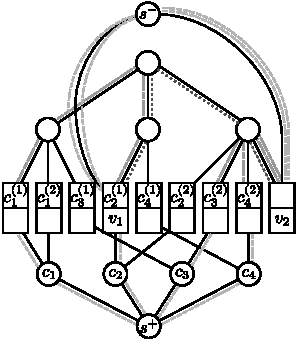
\includegraphics[width=\columnwidth]{figs/flow_ma_cv}
\caption{Example of flow construction: Problem instance with two virtual machines, four chunk
types, and two replicas per type. The min-cost-max-flow
is indicated by the dotted lines: each line represents one unit of flow.}
\label{fig:flow_construction}
\end{figure}

\textbf{Algorithm.}
Our algorithm to solve $\RS+\MA+\CC+\BW$ consists of three parts:
\emph{First}, we construct the normalized and extended graph $\Tree^*$ 
described above and compute
a min-cost-max-flow solution, e.g., using~\cite{mincostmaxflow-1,mincostmaxflow-2}.
\emph{Second}, we have to \emph{round} the resulting, possibly fractional flow, to
integer values. Due to the \emph{integrality theorem}~\cite{mincostmaxflow-1,mincostmaxflow-2},
there always exists an optimal integer solution on graphs with integer capacities.
However, while algorithm like the successive shortest path algorithm~\cite{successive_shortest_path_complexity}
directly give us such an integral solution (in polynomial time), the state-of-the-art min-cost-max-flow algorithms (e.g., based on double-scaling
methods~\cite{mincostmaxflow-1} or minimum mean-cost cycle algorithms~\cite{mincostmaxflow-2}), may yield fractional solutions
which need to be rounded to integral solutions (of the same cost). 
In order to compute integral solutions, we proceed as follows: we iteratively pick an arbitrary (loop-free) path 
currently having a fractional allocation of size $f$ ($f\in (0,1)$), and distribute its flow $f$ 
among all other fractional paths of the same length; due to the optimality of the fractional solution
and due to the integrality theorem, such paths must always exist. After distributing this flow,
the total allocation on this path will be 0, and we have increased the number of integer paths by one.
(In addition, some paths may now have an integer allocation of 1.) We proceed inductively. 
\emph{Third}, given an integer min-cost-max-flow solution, we need to decompose the integer flows into the paths
representing matched chunk-node pairs:
The assignment can be obtained be decomposing the flow allocated in the
original substrate network. In order to identify a matched chunk-node pair, 
we take an arbitrary (loop-free) path $p$ from $\Source$ to $\Sink$:
the first hop represents the chosen chunk type, the second hop the chosen
replica, and the last but one hop represents the server: we will assign
the replica to an arbitrary unused node on this server. 
Having found this matching pair, we remove the flow 
along the path $p$ by one unit.
We continue building the assignments by selecting replicas until every chunk type is processed.

\textbf{Analysis.}
The correctness of our approach follows from our construction
of $\Tree^*$, using integer capacities (in our case $\lfloor\capacity(e)/\CostTrans\rfloor$),
and the fact that cost optimal integer solutions always exist~\cite{mincostmaxflow-1,mincostmaxflow-2}.
The runtime of our algorithm consists of four parts: construction of $\Tree^*$,
computation of the min-cost-max-flow, flow rounding, and decomposition. The 
dominant terms in the asymptotic runtime is the flow computation.
The state-of-the-art min-cost-max-flow algorithms~\cite{mincostmaxflow-1} resp.~\cite{mincostmaxflow-2}
take time $O((n_S+\tau)^2 \log \delta \log\log U)$ resp.~$O(n_S^5 \cdot \tau^3 \log n_S)$, where $\delta$ is the 
network diameter and where $U$ is the maximal link capacity in the substrate.
\stefan{TODO: Carlo: actually the maximal link cost is 1, no?}

%\textbf{Summary.}
%Figure~\ref{fig:venn_flow} summarizes all problem
%variants which can be solved with our flow-based approach.

TODO: what about multiple nodes what about multiple replicas?

\subsection{Matching Algorithms ($\RS+\MA+\CC$ and $\MA+\CC+\BW$)}\label{ssec:match}

\begin{wrapfigure}{r}{0.5\columnwidth}
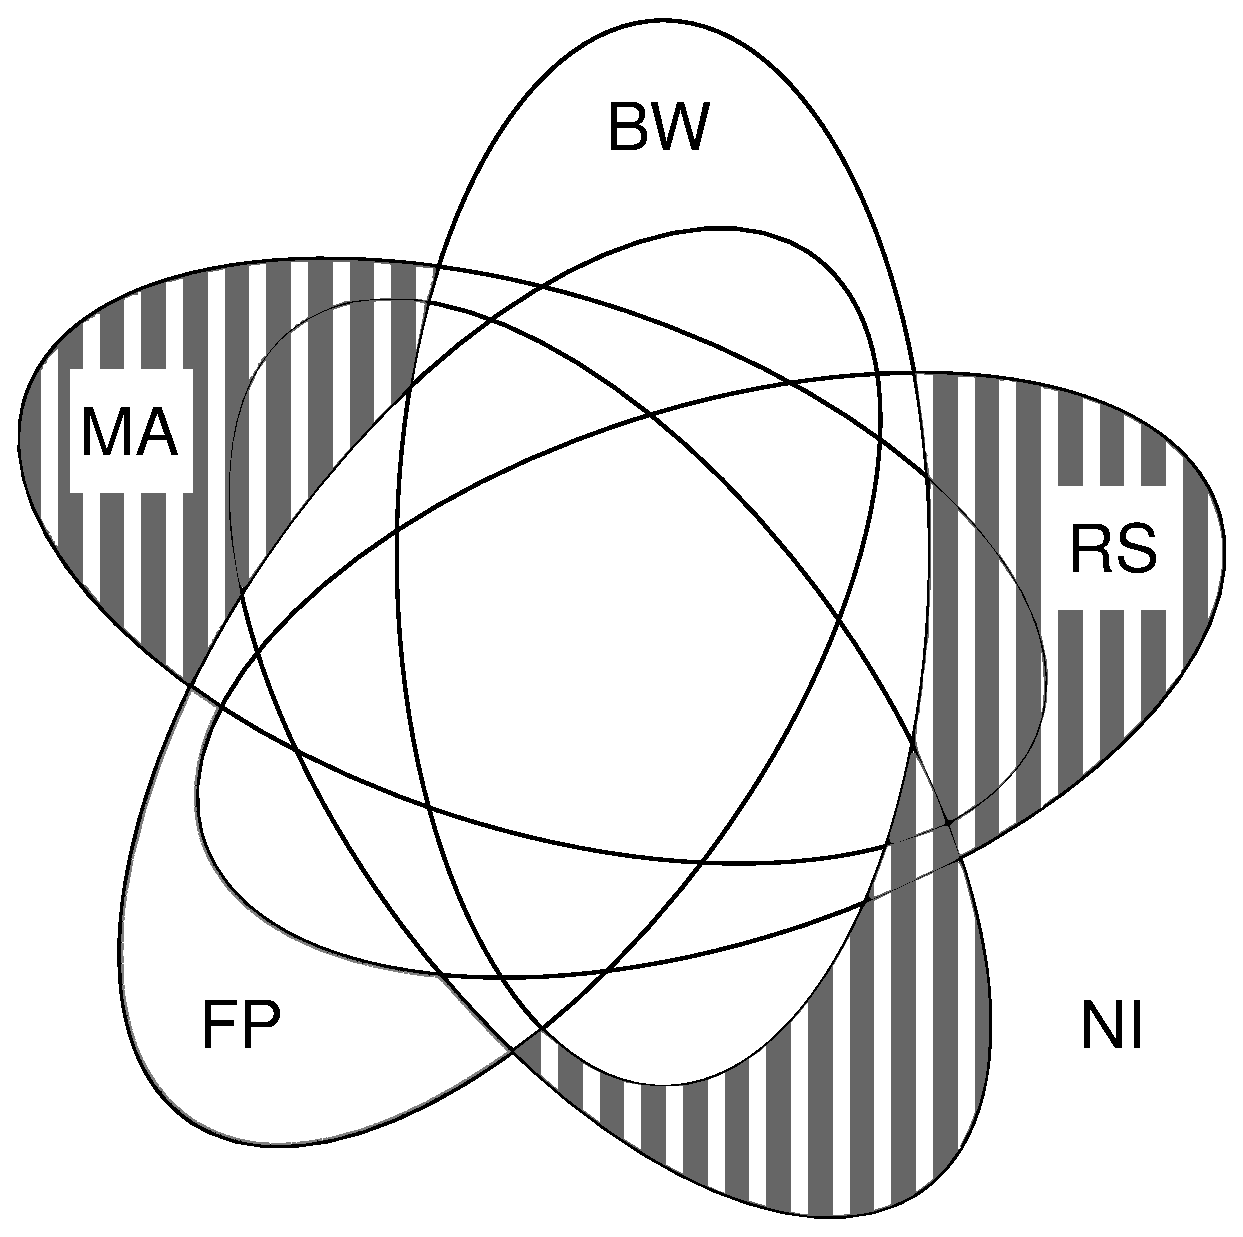
\includegraphics[width=0.48\columnwidth]{figs/venn_matching.pdf}
\caption{Variants solved by matching approach.}
\label{fig:venn_match}
\end{wrapfigure}

This section tackles the two problem variants
$\RS+\MA+\CC$ and $\MA+\CC+\BW$. In particular, we show that
for these problems, fast algorithms exist.
In general, the algorithms presented in this section can be summarized
as matching approaches.

\subsubsection{$\RS+\MA+\CC$}

Let us first consider the $\RS+\MA+\CC$ variant.
Recall that in this problem,
we are given a set of redundant chunks ($\RS$) and a set of virtual machines
at fixed locations. The number of chunk types is larger than the number
of virtual machines ($\MA$), and each virtual machine needs to be connected
to its chunks as well as to other virtual machines ($\CC$).
Our goal is to minimize the resource footprint $\Cost$, consisting
of the bandwidth reservations in the access network and the inter-connect.

\textbf{Algorithm.} Recall that $\RS+\MA+\CC$ degenerates to $\RS+\MA$,
in the absence of flexible placements. 
In order to solve the $\RS+\MA$ problem variant,
we construct a bipartite
graph between the set
$\VirtualNodes$ of nodes and
the set of chunks.
Concretely, we clone each node $\MaFactor$ times,
as each node needs to process
$\MaFactor$ replica types, and we collect all copies of a given chunk type in a
single %$\ChunkType$
``super-node''. We connect each node to all chunk types using the
\emph{lowest hop count} to one of the copies as the cost metric (the link weight).

On the resulting graph, we can now compute a \emph{Minimum Weight
Perfect Bipartite
Matching}:
the resulting matching describes the optimal assignment of chunks to nodes.

%\begin{figure}[h]
%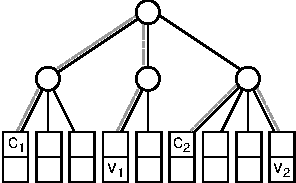
\includegraphics[width = 0.49\columnwidth]{figs/matching_topology_simple}
%\hfill
%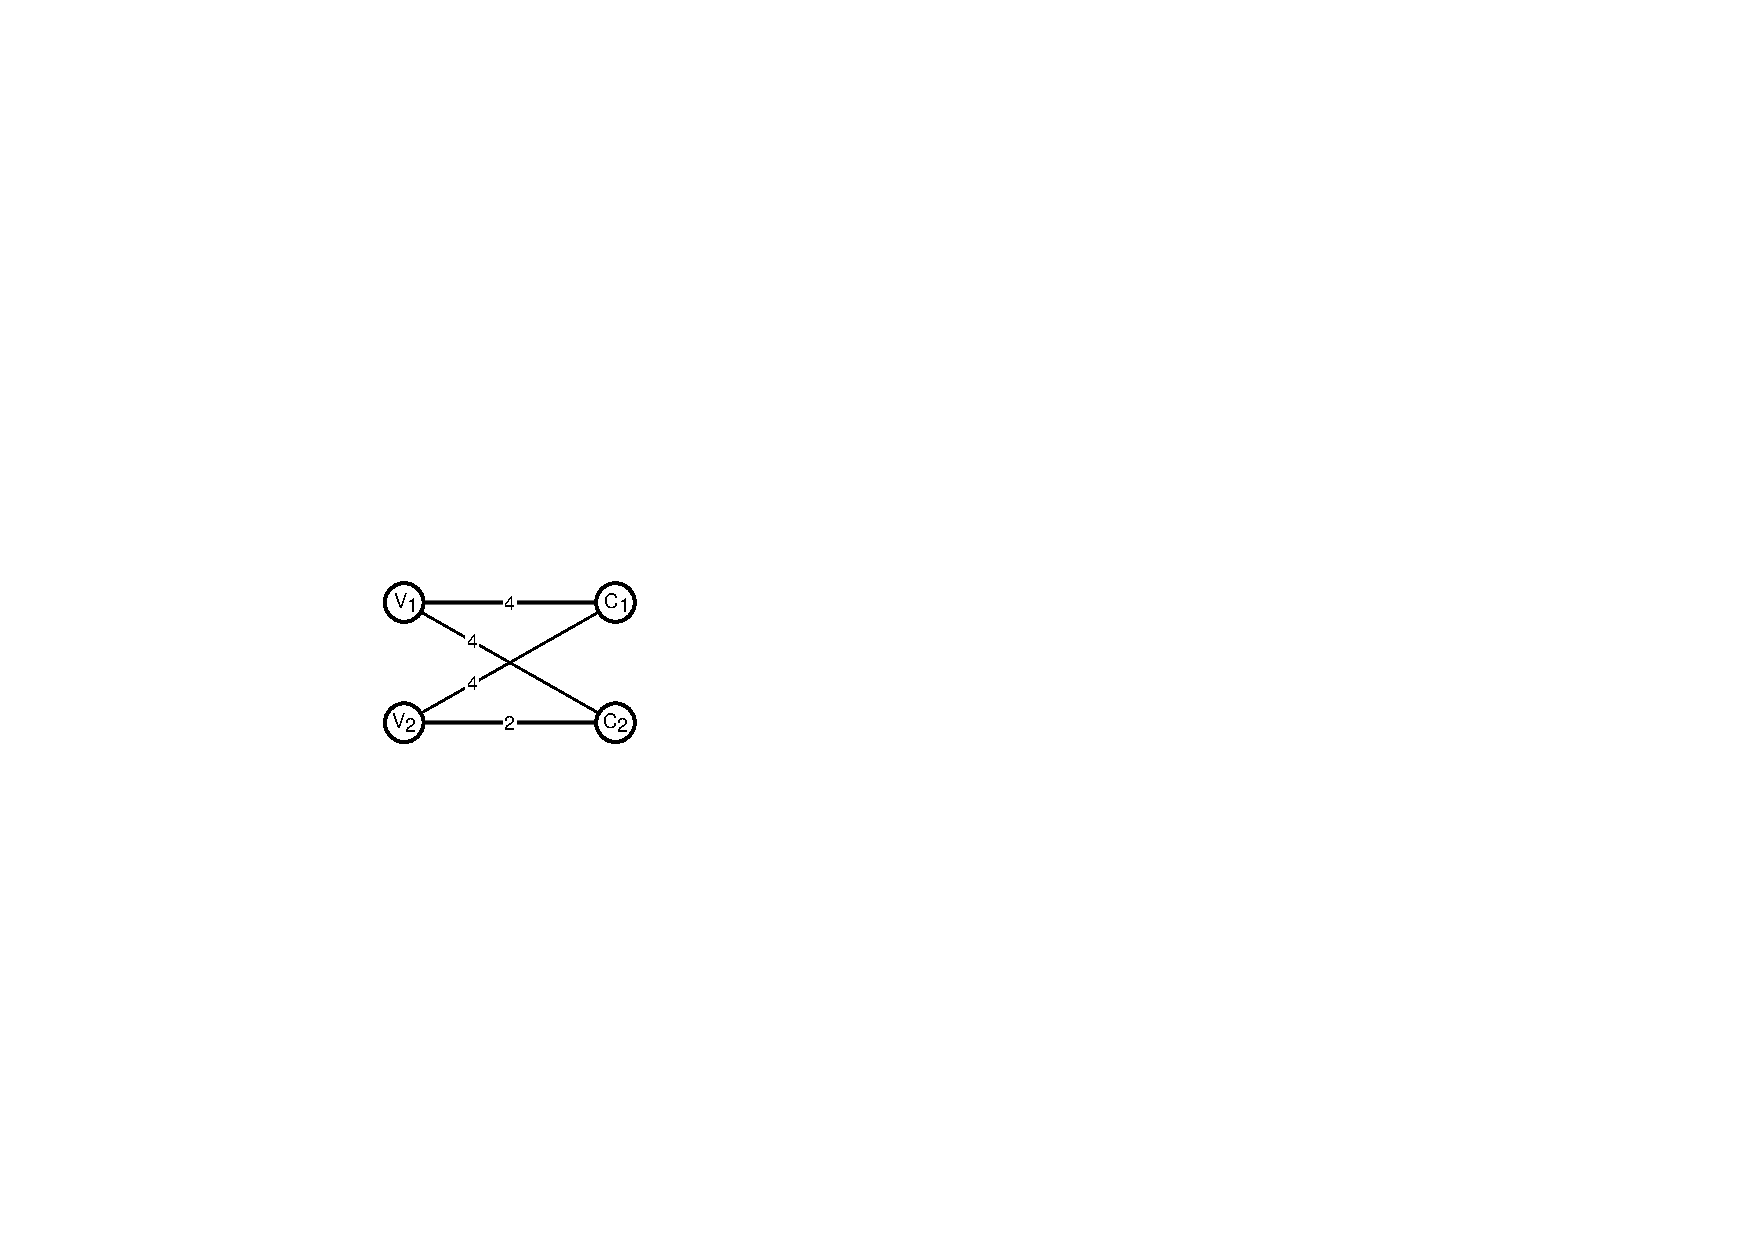
\includegraphics[width =0.4\columnwidth]{figs/matching_basic}
%\caption{The problem instance on the \emph{left} consists of
%two nodes and two chunks. The
%optimal solution is indicated by the dashed lines. The corresponding matching
%problem on the \emph{right} represents the same situation. The weights on the
%edges
%are set according to the distance in the substrate. The solution of the minimum
%cost perfect matching is depicted by the shaded lines.}
%\label{fig:matching_basic}
%\end{figure}

\begin{figure}
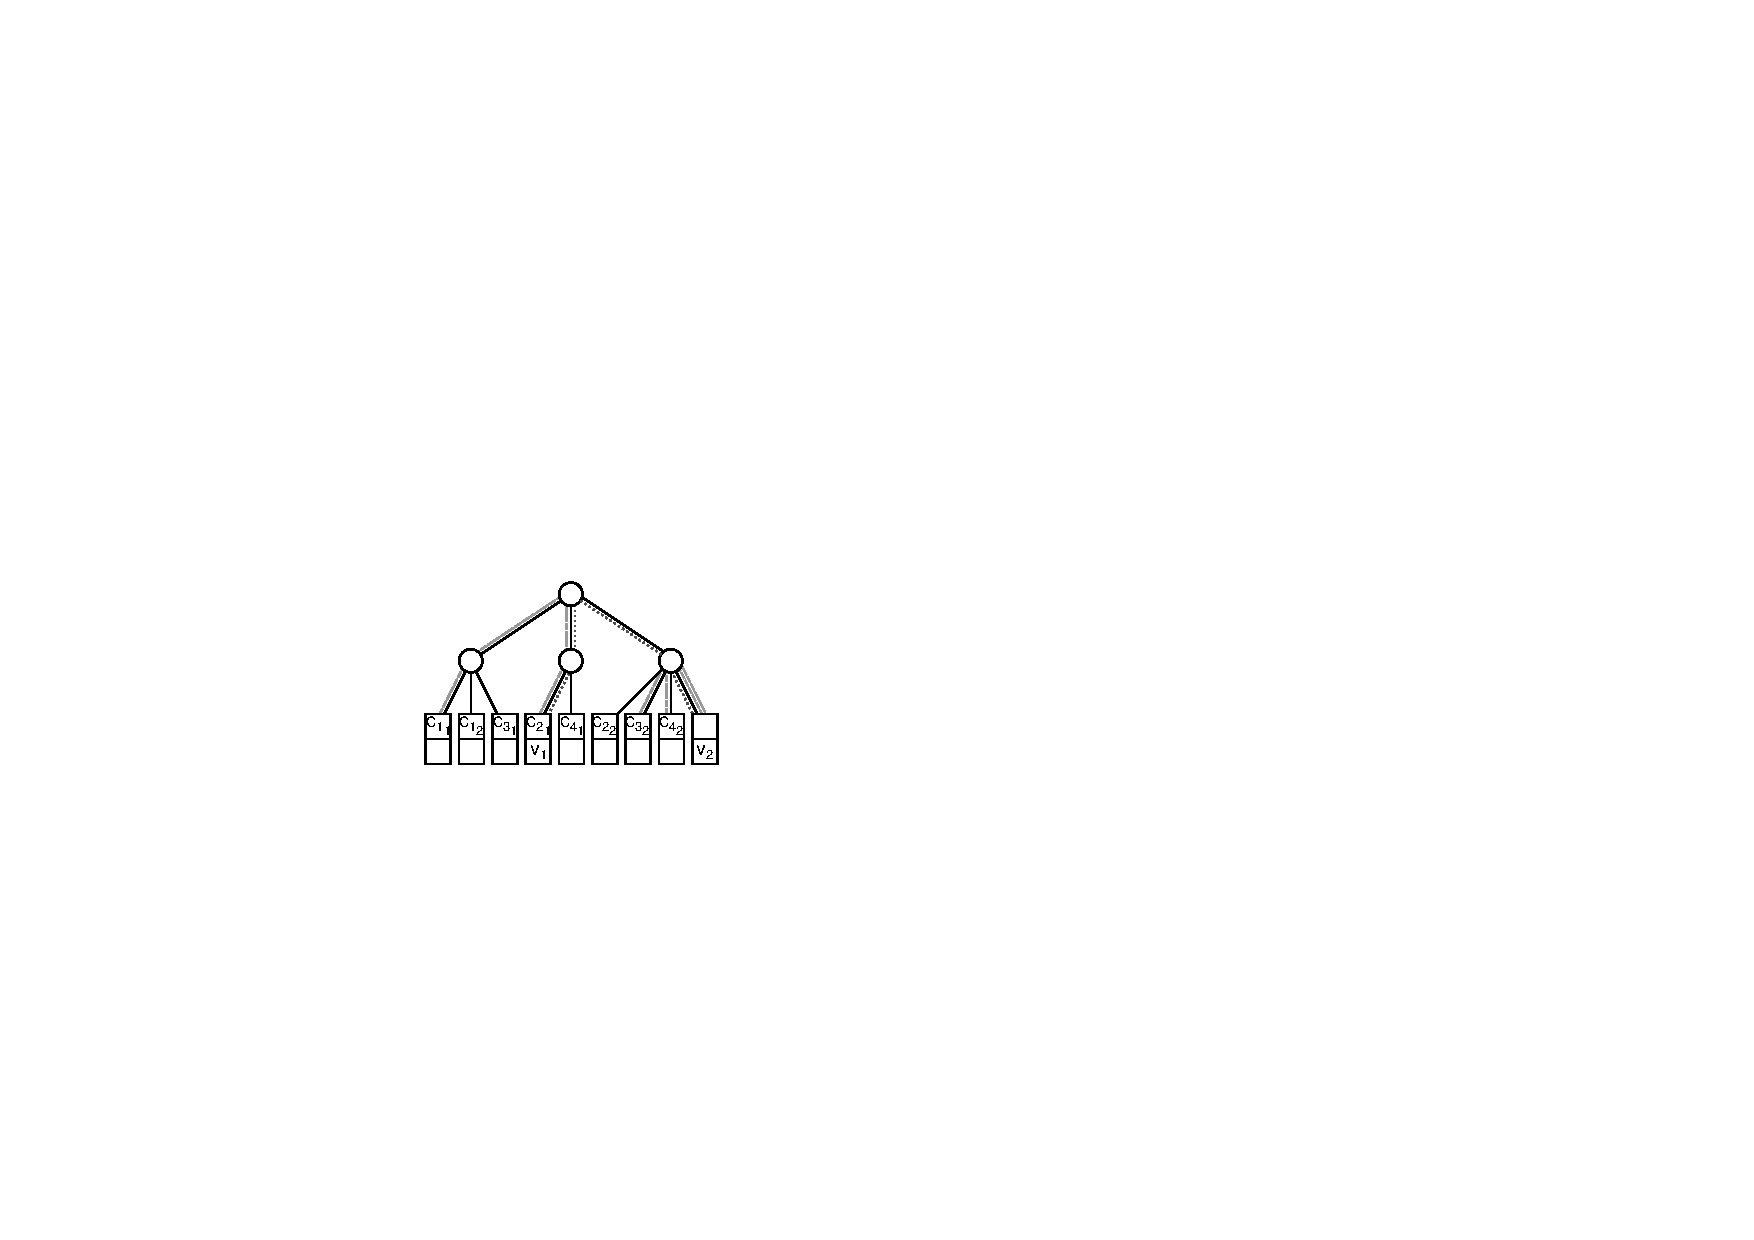
\includegraphics[width = 0.49\columnwidth]{figs/model_ma_r_cv_boxes}
\hfill
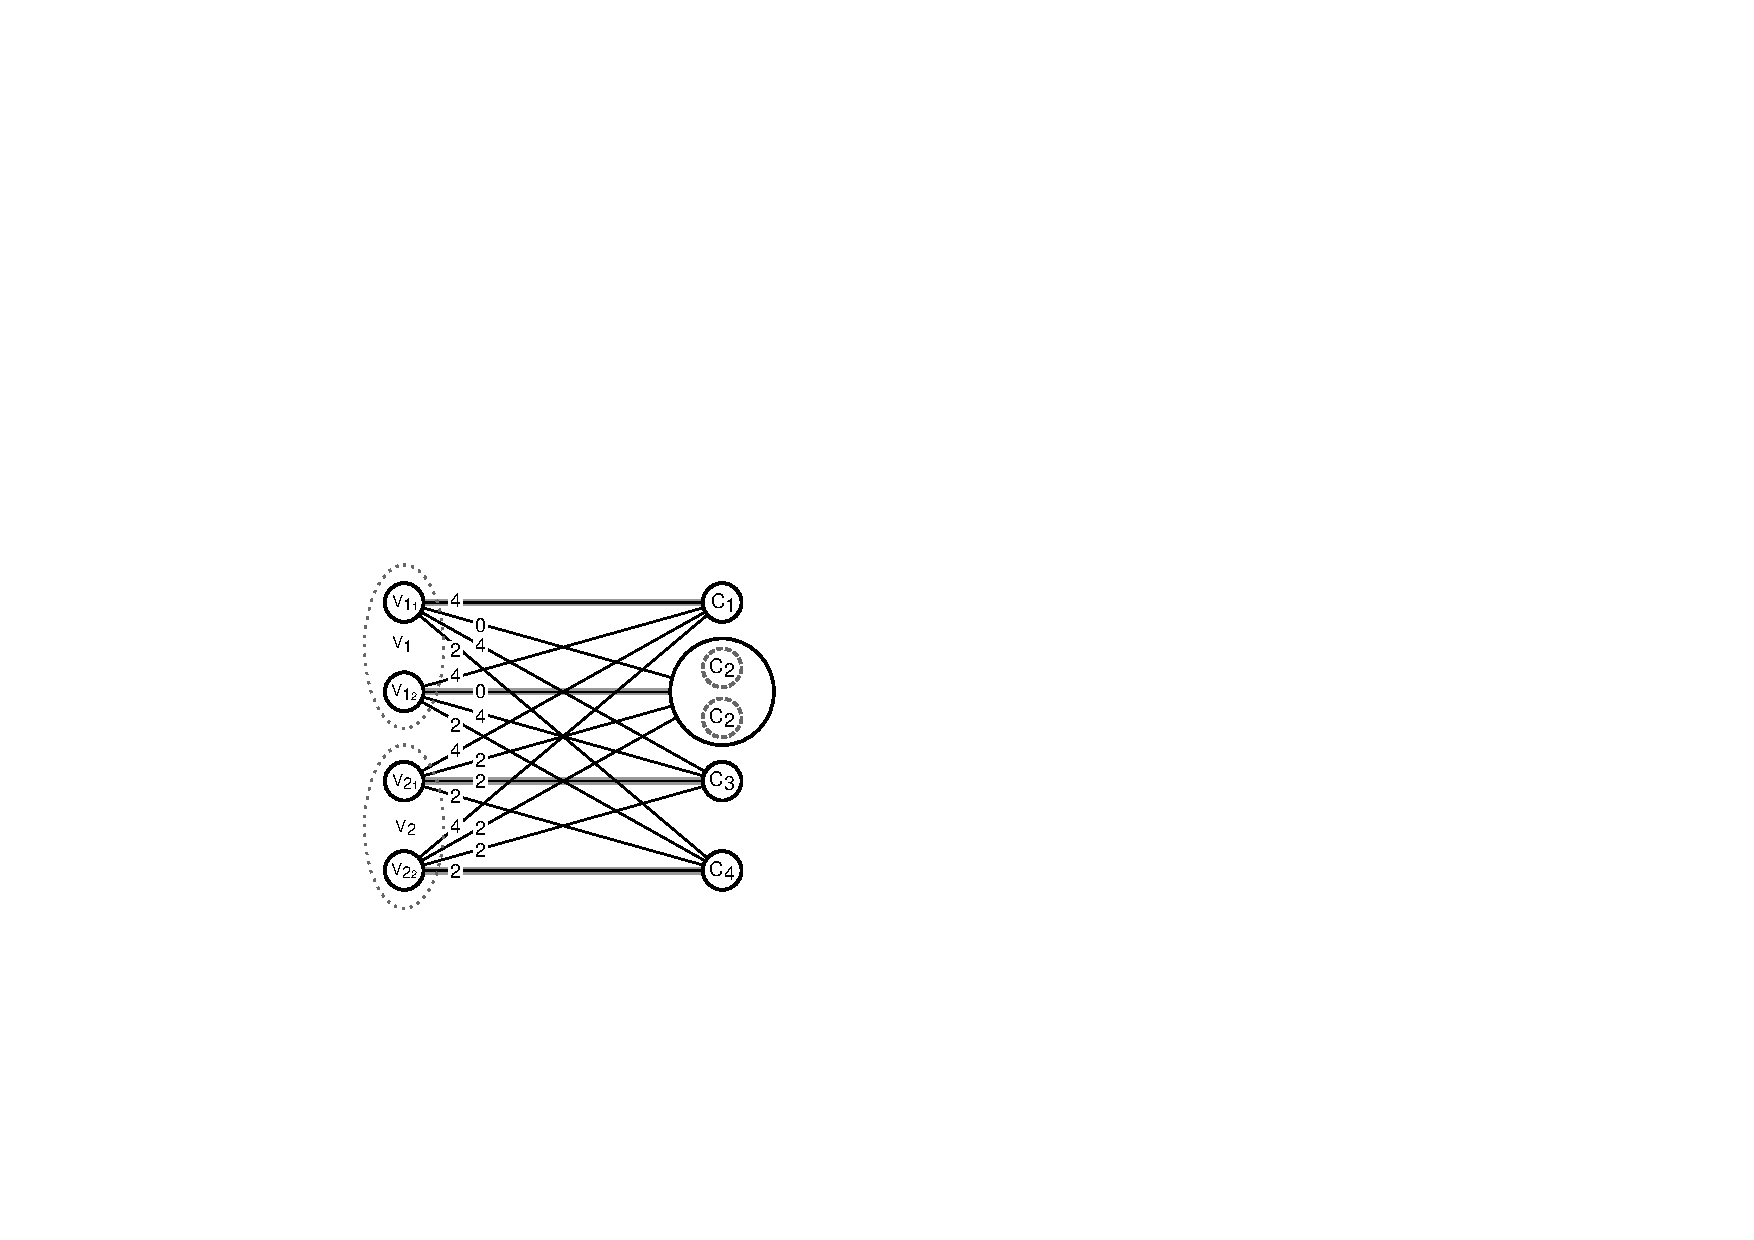
\includegraphics[width =0.49\columnwidth]{figs/matching}
\caption{The $\MA+\RS$ problem on the \emph{left} is converted into a
matching problem on the \emph{right}. Since each node has to process two
chunks, the
nodes are replicated in the matching representation. The two replicas of each
chunk type are represented by a single node, and all edges connecting to this
node have a weight according to the shorter distance to one of the replicas.
This is visualized for $\achunk_2$.}
\label{fig:matching}
\end{figure}

\textbf{Example.} Before analyzing our algorithm, let us consider a small example.
%
%Figure~\ref{fig:matching_basic} shows an example:
%$\NodeMapping(\VirtualNode_1)$ is four hops
%away from all chunks; in the matching problem, this is
%reflected in the corresponding edge
%weights. Similarly, $\NodeMapping(\VirtualNode_2)$ is
%two hops away from $\achunk_2$, and four hops away from $\achunk_1$. Hence the
%weight of the edge $(\NodeMapping(\VirtualNode_2),\achunk_2)$ is $2$, while the
%weight on the edge to $\achunk_1$ is $4$. The solution to the minimum weight
%perfect bipartite matching contains the edges $(\NodeMapping(\VirtualNode_1),
%\achunk_1)$ and $(\NodeMapping(\VirtualNode_2),
%\achunk_2)$, which is exactly the optimal chunk to node assignment
%$\VmChunkAssignment$,
%visualized using dashed lines in Figure~\ref{fig:matching_basic}.
%
%\begin{figure}
%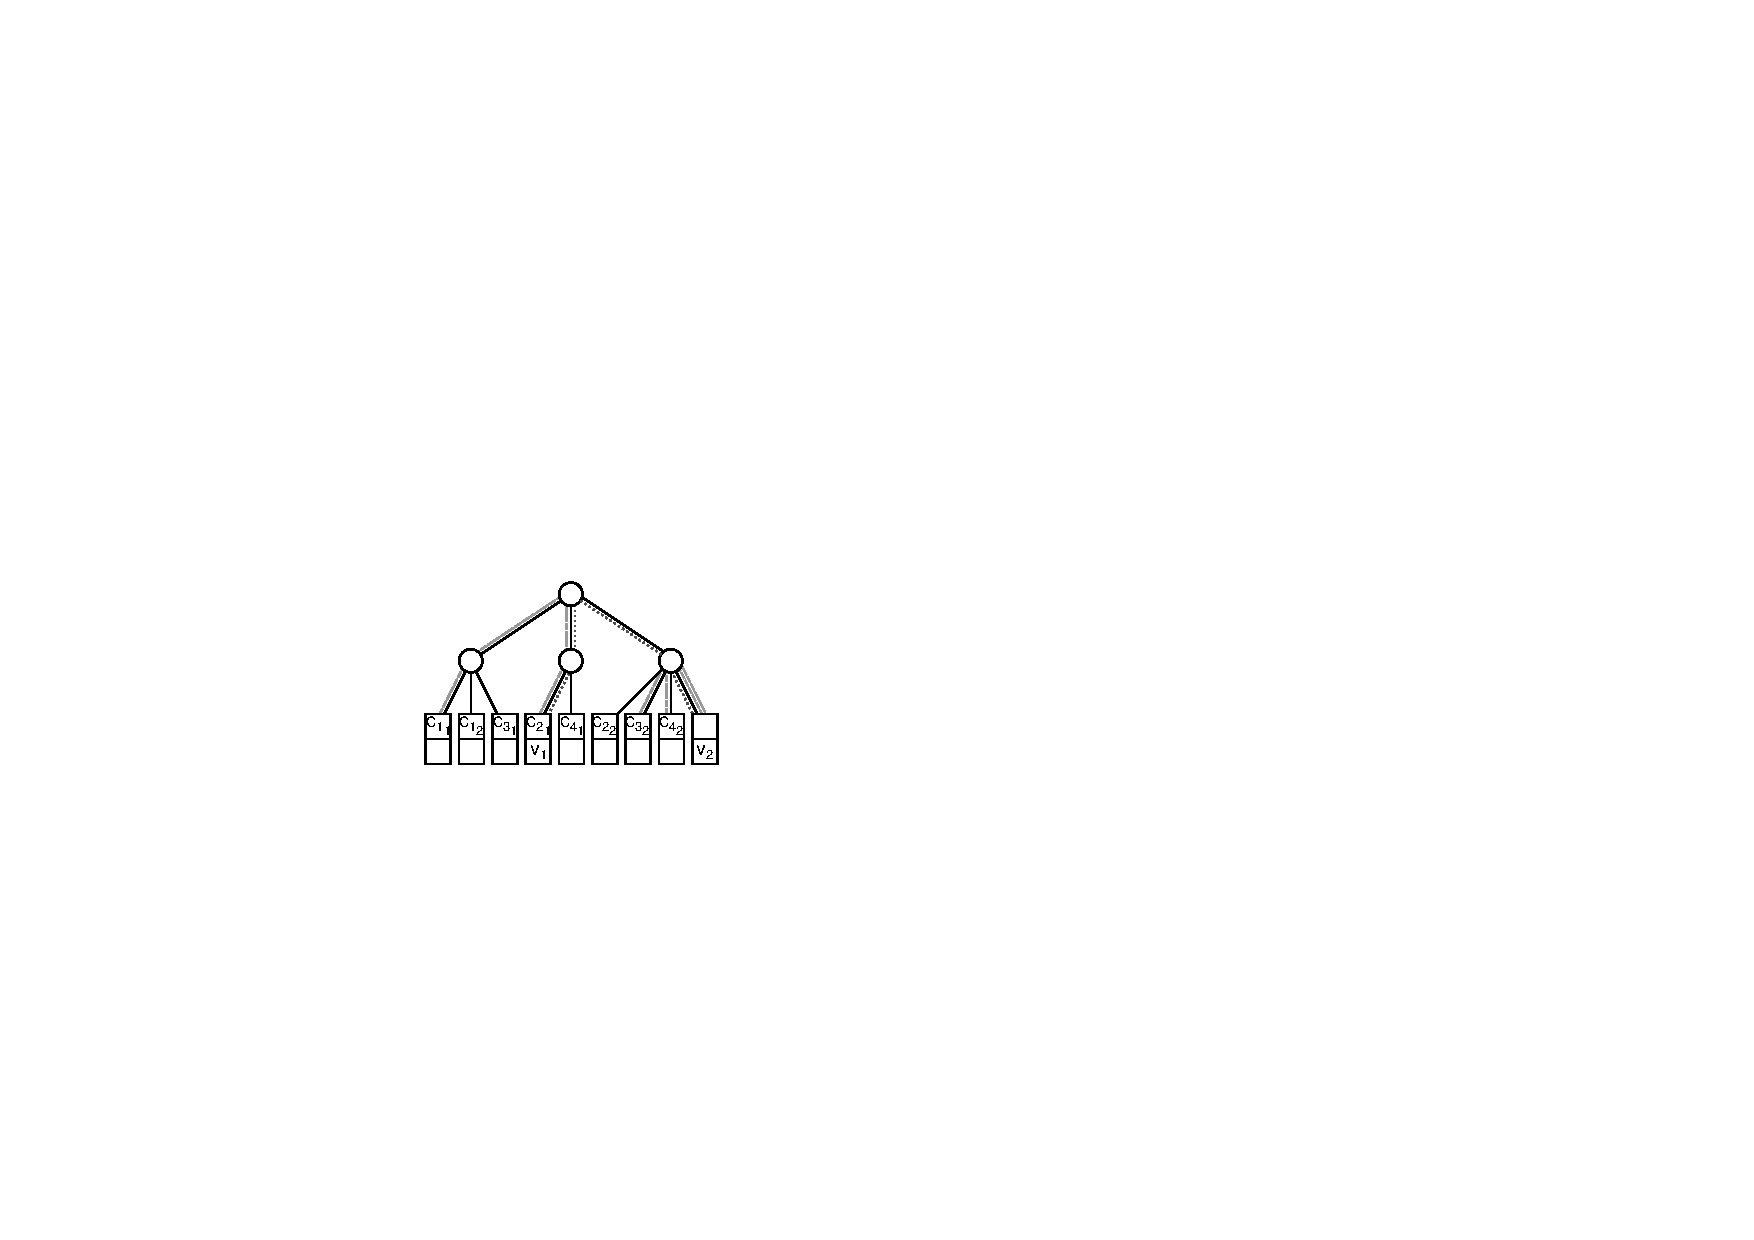
\includegraphics[width = 0.49\columnwidth]{figs/model_ma_r_cv_boxes}
%\hfill
%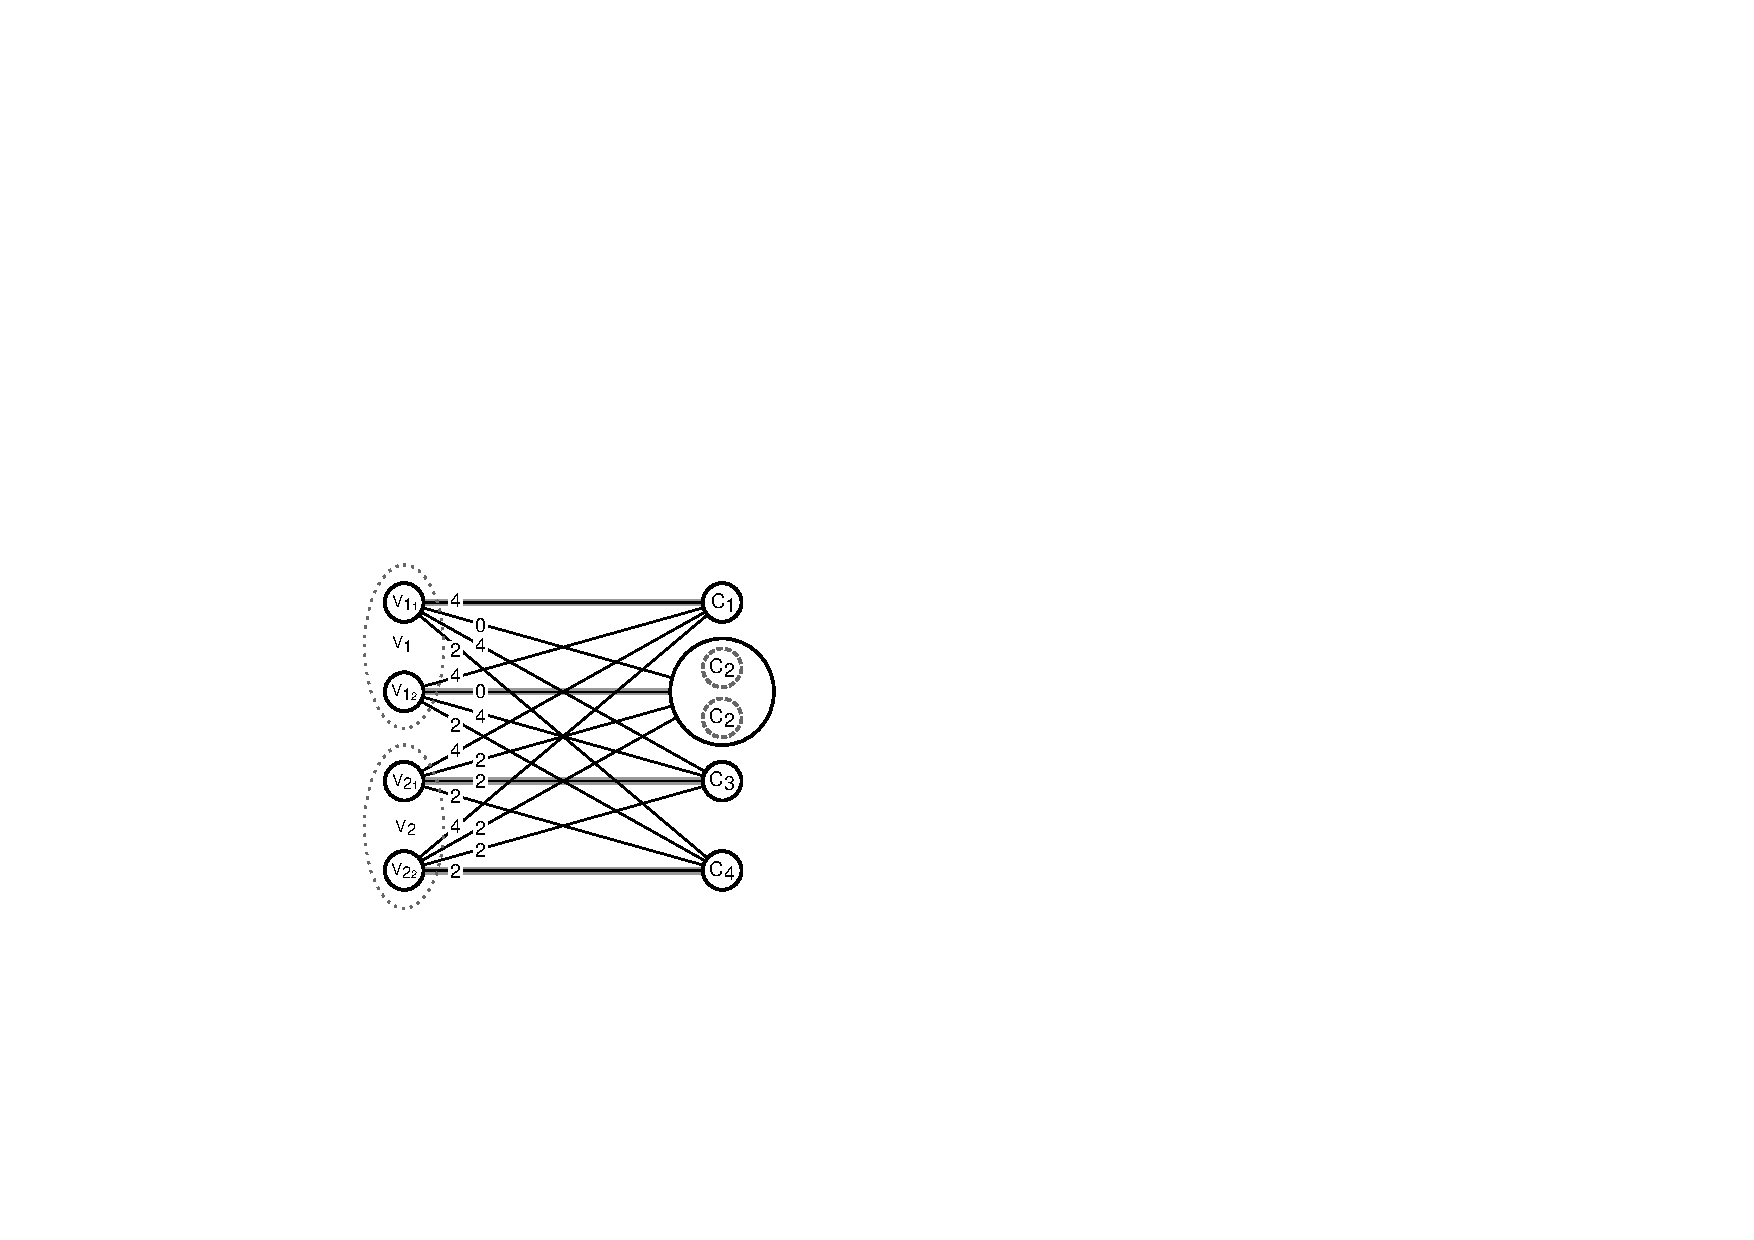
\includegraphics[width =0.49\columnwidth]{figs/matching}
%\caption{The $\MA+\RS$ problem on the \emph{left} is converted into a
%matching problem on the \emph{right}. Since each node has to process two chunks, the
%nodes are replicated in the matching representation. The two replicas of each
%chunk type are represented by a single node, and all edges connecting to this
%node have a weight according to the shorter distance to one of the replicas.
%This is visualized for $\achunk_2$.}
%\label{fig:matching}
%\end{figure}
%
Figure~\ref{fig:matching} illustrates
%the procedure for a more complex problem
an instance where two nodes are
cloned into $\MaFactor = 2$ nodes each, resulting in a total of four nodes in
the matching problem representation.
The $\RedundancyFactor = 2$ chunks of each chunk type are
aggregated into a single chunk type node $\achunk_j$  in the matching problem;
this gives a total of four chunk type nodes in the matching graph. The costs
on the links between all clones of a specific node and a chunk type are set to
the minimum distance. This can for instance be observed at the edges connecting
the two clones of $\VirtualNode_1$ to $\achunk_2$: both weights are 0.

\textbf{Analysis.}
%Let us now study the runtime of the matching approach.
The correctness of our algorithm follows from the construction and the optimal
solution of the minimum matching. 
The runtime consists of two parts: the construction of the matching graph and
the actual matching computation. The constructed graph consists of
$\MaFactor \cdot n_V \cdot \ChunkType$ many edges,
and for each edge we need to compute its cost, i.e., the shortest distance
which can be computed in time $n_S$; thus, the overall construction time
is $O(n_S \cdot \MaFactor \cdot n_V \cdot \ChunkType)$.
The state of the art algorithm to compute matchings are due to Gabow et al.~\cite{gabow_scaling_algorithm}
and are based on scaling techniques. 
Its runtime translates to 
%graph $n$, the number of edges in the graph $m$, and the largest magnitude of
%an edge weight $N$. An efficient algorithm is described by Gabow et al. in
%\cite{gabow_scaling_algorithm} and provides a runtime of 
%$\mathcal{O}(n_S^{3/4} \cdot \lambda \cdot \log \delta)$, where $\delta$ is the network diameter
%and where $\lambda= \MaFactor \cdot n_V \cdot \ChunkType$ represents the number of edges in the matching graph.
$\mathcal{O}(\tau^{11/4}*n_S)$, which dominates the asymptotic runtime. (Recall that $\tau = \MaFactor\cdot n_V$.)

\stefan{todo: doublecheck!!}

\begin{comment}
The following lemma essentially states that any non-local matching can only have higher
costs in all subtrees.

\maciek{We need to introduce what we mean by partial matching before
  formulating this lemma.}
\begin{lemma}\label{lemma:local}
A local and greedy perfect matching of chunks to nodes is optimal.
\end{lemma}
\begin{proof}
Proof by contradiction. Let us assume that there exists an optimal matching $M'$ of cost lower
than the local greedy matching $M$.
Let us consider the smallest subtree where the (partial) matching of $M$
has a different cost than the (partial) matching of $M'$.
This means
that a non-local decision was made by $M'$ in this subtree (hoping for savings higher up),
and there must exist two matched pairs in $M'$ that shares a link (one pair is transporting a chunk up, and
 the other one a chunk down). Then we can create a matching $M''$
 which uncrosses these edges of $M'$ (i.e., does the local matching on them),
  and is cheaper than $M'$. Contradiction.
\end{proof}

\end{comment}

\subsubsection{Faster $\MA+\CC$ and $\MA+\CC+\BW$}

We will now show that faster algorithms exist for $\MA+\CC$, by exploiting
locality. Moreover, we will show that
even
$\MA+\CC+\BW$ problem variants can be solved with our approach, by simply
verifying feasibility.
Let us also recall that we can ignore $\CC$ and focus on the $\MA$ resp.~$\MA+\BW$ problem, 
as it is constant
without $\FP$.

We first need the following definition.
\begin{defn}[Local Assignment (LA)]\label{def:loc}
We define an assignment $\VmChunkAssignment$ to
be \emph{local in a specific subtree $\Tree'$}, iff.~$\VmChunkAssignment$
assigns the maximum number of chunks in the
subtree to nodes in the same subtree.
% (subject only to the number of available nodes
%in $\Tree'$). 
We define $\VmChunkAssignment$ to be \emph{local} when
it is local with respect to all all possible subtrees of the substrate network.
\end{defn}

We will see later that 
optimal solutions to
$\MA+\CC$ have a local assignment. This is exploited by our algorithms described in the following.

\textbf{Algorithm.} Our proposed algorithm for $\MA$ 
proceeds in a bottom-up fashion, traversing the substrate network $\Tree$
from the leaves toward the root.
For each subtree $\Tree'$, we maintain
two sets $S_1,S_2$ in order to match unmatched
chunks $S_1$ in the subtree $\Tree'$ to unmatched 
nodes $S_2$ in $\Tree'$. Both sets are initially empty.

We first process all the leaves, in an arbitrary order; subsequently, we process arbitrary inner vertices
of $\Tree$, whenever all their children have been processed. 
We process any leaf $\ell$
by adding any
nodes or chunks which are located on $\ell$ to the corresponding sets $S_1$ and $S_2$. 
A non-leaf vertex $vu$ is processed in the following way: we take the union of
the sets of $u$'s children, i.e., the sets contain the unmatched chunks and nodes
in this subtree. 
For both leaf and inner nodes, whenever
both sets are non-empty, we greedily match an arbitrary chunk in $S_1$ with an arbitrary chunk in $S_2$,
and remove them from the sets.

\textbf{Analysis.} On a given vertex $u$, emptying one of the sets, results in a \emph{local assignment} (cf~Definition~\ref{def:loc})
in the
subtree rooted at $u$. Due to our bottom-up strategy, the overall assignment
will also be local. 
The complexity of this
construction is low: Each
vertex in the substrate graph has to be processed once (runtime
$\mathcal{O}(|\SubstrateNodes|)$). The sum of all remove operations, is equal to
the number of chunks $\mathcal{O}(\ChunkType)$. Verifying that all children
which have
been processed can be done in constant time, leveraging a counter on the parent
node. Hence the overall complexity of this construction is
$\mathcal{O}(|\SubstrateNodes| + \ChunkType)$.

It remains to prove optimality of such local assignments.
We first characterize the bandwidth allocation on uplinks of subtrees.
\begin{lemma}\label{lem:uplink-alloc}
Given an $\MA$ problem and a subtree $\Tree'$
containing $x$
chunks and $y$ nodes, the bandwidth allocation of each local assignment
$\VmChunkAssignment$ on the uplink of $\Tree'$ is $|x-(y\cdot\MaFactor)|\cdot
\CostTrans$.\label{lemma:uplink}
\end{lemma}
\begin{proof}
Clearly, if the number of chunks equals the number of nodes in a subtree,
the $\CostTrans$-inflicted bandwidth allocation at the uplink is zero in a local
assignment. 
Otherwise, we distinguish between two cases: In case
there are more chunks in the subtree, each
excess chunk has to be transferred to a different subtree, which will
inflict costs $\CostTrans$ on the uplink connecting $\Tree'$ with the
remaining parts of $\Tree$. Similarly, if the processing capabilities exceed the
amount of
available chunks, chunks from other subtrees will have to be transferred to
nodes in the subtree $\Tree'$, inflicting bandwidth costs of $\CostTrans$ each.
Hence, the bandwidth allocation for the chunk transport on the uplink is the 
difference between the number of chunks and the processing capabilities of
the subtree $|x-(y\cdot\MaFactor)|$ times the amount of bandwidth needed, for a
single transfer $\CostTrans$.
\end{proof}

Since each link is an uplink of one subtree,
Lemma~\ref{lem:uplink-alloc} implies:
\begin{corollary}
All local assignments result in the same cost, for any $\CC+\MA$ problem instance.
\label{corollary:same_costs}
\end{corollary}

\stefan{TODO: add unbalanced tree pic}

We can now prove optimality: 
\begin{theorem}
Given an $\CC+\MA$ problem instance, a feasible assignment $\VmChunkAssignment$
is optimal iff it is local.
\label{thm:local_optimal}
\end{theorem}
\begin{proof}
By contradiction. We will show, that a non-local assignment is not optimal. Combined with
Corollary~\ref{corollary:same_costs}, this results in the optimality of all
local assignments.

Assume a non-local optimal assignment $\VmChunkAssignment$ exists. 
This means, for at least one subtree, it assigns
a chunk $\achunk_i$, located in the subtree, to a node $\VirtualNode_i$ outside
the
subtree. In addition,
at least one node $\VirtualNode_j$ in the subtree has to process a chunk
$\achunk_k$ located outside the subtree. We construct an alternative
assignment $\VmChunkAssignment'$, by exchanging the assignments of
$\achunk_i$ and $\achunk_j$. Since $\achunk_i$ is located in a subtree which
contains $\VirtualNode_j$ but not $\VirtualNode_i$, and both nodes and chunks
are only located at leaves, the distance between $\achunk_i$ and its assigned
node is smaller in $\VmChunkAssignment'$. For the distance between $\achunk_j$
we make a case distinction: if there exists a subtree which
contains $\achunk_i$, $\achunk_j$ but not $\VirtualNode_i$, the distance
between $\achunk_i$ and $\VirtualNode_i$ is equal to the distance between
$\achunk_j$ and $\VirtualNode_i$. Since $\achunk_i$ is closer to
$\VirtualNode_j$ than $\achunk_j$, the overall costs of $\VmChunkAssignment'$
would be lower in this case. If the described subtree does not exist, the
distance between $\achunk_j$ and the two nodes is the same, which 
renders $\VmChunkAssignment'$ cheaper than an optimal
solution. Contradiction.
\end{proof}

Combined with a simple postprocessing, this approach can also solve $\MA+\BW$
(and therefore $\MA+\BW+\CC$). The central idea of this extension, is to show
that if the \emph{local} assignments violates the available bandwidth on any
link, all other assignments will also violate the bandwidth. As a consequence
it is possible to simply compute the assignment without any bandwidth constraints, and
check in a postprocessing step, whether the bandwidth on any link is exceeded.
This postprocessing step scales with the number of edges in the substrate,
which is lower than the number of nodes in the substrate. 
Hence the asymptotic runtime of the approach does not change.


\stefan{fix the following! also note that the notation $F(...)$ has not been introduced!}

\begin{lemma}
Given a minimal cost assignment $\VmChunkAssignment$,
any solution with bandwidth allocation less
than $\Cost(\VmChunkAssignment,
\SubstrateEdge)$ to any link renders the problem
infeasible.
\label{lemma:no_bandwidth}
\end{lemma}
\begin{proof}
\maciek{This proof is too slippery! Simpler way to proof that surely exists.}
From Lemma~\ref{lemma:uplink} we know that each optimal assignment
$\VmChunkAssignment$ to $\MA+\CC$ assigns a certain bandwidth to a link. This is
the minimal bandwidth which has to be allocated on this link by \emph{any}
feasible assignment, since removing the locality, can only increase the number
of chunks which have to be transported across the uplink.
Assume there exists a link on which the assignment $\VmChunkAssignment$
violates the capacity. Since $\VmChunkAssignment$ allocated the minimal
bandwidth on this link, which has to be allocated by \emph{any} feasible
assignment, the problem has to be infeasible.
\end{proof}


\begin{comment}
\subsubsection{$\MA+\CC+\BW$}

We can also solve the $\CC+\MA+\BW$ problem variant with our matching approach.
The algorithm
essentially uses
the same construction described above for $\CC+\MA$ (but without $\RS$) to
compute a solution
to minimum weight perfect matching. Afterwards it is verified whether the
resulting bandwidth allocations satisfy capacity constraints. If
no capacities are violated, we found the cheapest assignment. We will
now show, that the problem is infeasible if the resulting assignment
violates capacity constraints of at least one link.
Before we can prove the infeasibility of the instances, we will
state the following lemma
which gives us a better understanding of the \emph{locality} of optimal
assignments.
\carlo{NEW VERSION STARTS HERE:}

\begin{lemma}
\label{lemma:local}
Given an instance of $\MA+\CC$ and an arbitrary subtree, an optimal assignment
$\VmChunkAssignment$, assigns all chunks in the subtree to nodes in the same
subtree (subject to the number of avialable nodes in the
subtree).\stefan{Can this stay this way?} \maciek{Why did we restate
  the local matching lemma (it is worse here)? And why are we rewriting working proof?}
\end{lemma}


\begin{proof}
\carlo{
By contradiction. Assume an optimal assignment $\VmChunkAssignment$ exists,
which assigns a chunk $\achunk_i$ to a node $\VirtualNode_i$ outside the
subtree, although there are sufficient nodes for all chunks in the subtree.
Then
at least one node $\VirtualNode_j$ in the subtree has to process a chunk
$\achunk_k$ located outside the subtree. We construct an alternative
assignment $\VmChunkAssignment'$, by exachanging the assignments of
$\achunk_i$ and $\achunk_j$. Since $\achunk_i$ is located in a subtree which
contains $\VirtualNode_j$ but not $\VirtualNode_i$, and both nodes and chunks
are only located at leaves, the distance between $\achunk_i$ and it's assigned
node is smaller in $\VmChunkAssignment'$. For the distance between $\achunk_j$
we have to do a case differentiation: if there exists a subtree which
contains $\achunk_i$, $\achunk_j$ but not $\VirtualNode_i$, the distance
between $\achunk_i$ and $\VirtualNode_i$ is equal to the distance between
$\achunk_j$ and $\VirtualNode_i$. Since $\achunk_i$ is closer to
$\VirtualNode_j$ than $\achunk_j$ the overall costs of $\VmChunkAssignment'$
would be lower in this case. If the described subtree does not exists, the
distance between $\achunk_j$ and the two nodes is the same - which would also
render $\VmChunkAssignment'$ cheaper than an optimal
solution.}\maciek{This proof only considers complete matchings, but we
need to show that property on partial matchings.}
\end{proof}




\carlo{We also need a node mapping (for both lemmas). Shall we state this here?}

\begin{lemma}
Given a $\CC+\MA$ problem instance and a subtree rooted at vertex $u$ containing $x$
chunks and $y$ nodes, the bandwidth allocation of each optimal assignment
$\VmChunkAssignment$ on the uplink of $u$ is $|x-(y\cdot\MaFactor)|\cdot
\CostTrans$.\label{lemma:uplink}
\end{lemma}
\begin{proof}
From the local lemma (Lemma~\ref{lemma:local}),
the optimal bandwidth allocation is given by
a ``local'' assignment, in which all chunks inside the
subtree are assigned to nodes in the subtree and vice-versa. However, the
number of chunks in the subtree may differ from the processing capacities of
the nodes in the subtree. In case there are more chunks in the subtree, each
excess chunk has to be transferred to a different subtree, which will
inflict bandwidth costs of $\CostCom$ on the uplink connecting $u$ with the
remaining parts of $\Tree$. Similarly, if the processing capabilities exceed the amount of
available chunks, chunks from other subtrees will have to be transferred to
nodes in the subtree of $u$, inflicting bandwidth costs of $\CostCom$ each.
Every solution
which does not provide this ``locality'' cannot be optimal, since a better
solution can be constructed, by exchanging the assignments of one of the chunks
which is transferred inside $u$'s subtree and one chunk which is transferred from
the subtree to a node outside.
\end{proof}

The optimality then follows from the following lemma.
\begin{lemma}
Given a minimal cost assignment $\VmChunkAssignment$,
any bandwidth function with a capaciy which is lower then the bandwidth
allocation of $\VmChunkAssignment$ on any link, renders the
problem infeasible.
\label{lemma:no_bandwidth}
\end{lemma}
\begin{proof}
Assume there exists a link on which the assignment $\VmChunkAssignment$
  \maciek{This proof is too slippery! Simpler way to proof that surely exists.}
violates the capacity. From Lemma~\ref{lemma:uplink} it is
known that $\VmChunkAssignment$ keeps the assignment ``local''.
Therefore, the footprint on the uplink of a specific subtree is the number of chunks
(or nodes) which have to be connected to nodes (or chunks) outside the subtree,
times the bandwidth which is necessary to transfer a chunk to a node. There
cannot be an assignment which requires less bandwidth on the link, since all nodes
and chunks have to be used in the assignment and removing the
locality will increase the bandwidth requirements.
\end{proof}
%\begin{lemma}
%An instance of $\Problem$ is infeasible iff. algorithm returns $\infty$.
%\end{lemma}
%\begin{proof}
%  ($\rightarrow$)
%
%  ($\leftarrow$)
%  \end{proof}
%
%\maciek{I think that we do not need that lemma, it might be obvious. I leave it
%there just in case.}
%\begin{lemma}
%  If algorithm returns solution $\Sol$ of cost $\neq \infty$, then in $\Sol$ no
%link exceeds its capacity limit.
%  \end{lemma}

\carlo{TODO: change notation of instance of chunk types.}

\begin{figure}
 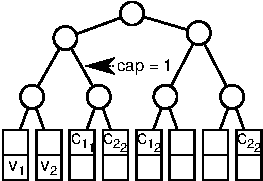
\includegraphics[width = \columnwidth]{figs/matching_no_rs}
 \caption{An example for the $\RS+\BW$ problem variant: $\achunk_{1_1}$ or $\achunk_{2_1}$ are
located in a subtree with uplink capacity $1$. The bandwidth allocation in the right
subtree depends on which chunk is chosen for processing in the left
subtree.}
 \label{fig:matching_no_rs}
\end{figure}


\textbf{Runtime.} While \carlo{minimum weight perfect} matching problems can be
solved in polynomial
time~\cite{schrijver_combinatorial_optimization} using
general algorithms, in the following, we show that for our problem
a simple and fast greedy strategy is sufficient.
Accordingly, we can use greedy bottom-up construction of matching.
Its runtime is linear with respect to number of tree vertices. It is more
efficient that more general methods of
finding perfect matching in general bipartite graphs.

\begin{corollary}
An optimal matching of nodes to chunks can be computed greedily, by
alternating selecting edges with the lowest cost and removing the chossen
edge, and all edges connected to the nodes of these edge.
\end{corollary}

\begin{proof}
Given an edge with the lowest costs, we can compute the smallest subtree, which
contains both, the node and the chunk which are connected by the edge. Since we
know that there is no node in a smaller subtree containing the chunk, we can
assign the node to the chunk, and according to Lemma~\ref{lemma:local}, the
resulting assignment will be optimal.
\end{proof}



Finally, let us observe that $\RS+\BW$ cannot be solved using this approach,
as Lemma~\ref{lemma:uplink} does not
hold for problem instances with $\RS$. Figure~\ref{fig:matching_no_rs}
illustrates this problem: It shows a feasible problem instance in which, due
to bandwidth constraints, only one chunk can be processed locally. If for
instance $\achunk_{1_1}$ is assigned to $\VirtualNode_1$, $\achunk_{2_1}$ cannot
be processed by $\VirtualNode_2$, since this would exceed the bandwidth
capacity. Instead $\achunk_{2_2}$ will be processed by $\VirtualNode_2$. This
requires bandwidth allocations on links, which would not have been utilized,
when $\achunk_{2_1}$ would have been assigned to $\VirtualNode_1$. Hence the
bandwidth utilization on individual links is no longer predictable in $\RS$.
When this problem is transformed into a matching problem, the resulting
assignment will use $\achunk_{1_1}$ and $\achunk_{2_1}$, which violates
bandwidth constraints, although the instance itself is feasible.

\textbf{Summary.}
Figure~\ref{fig:venn_match} summarizes all problem
variants which can be solved with our flow-based approach.
\begin{wrapfigure}{r}{0.5\columnwidth}
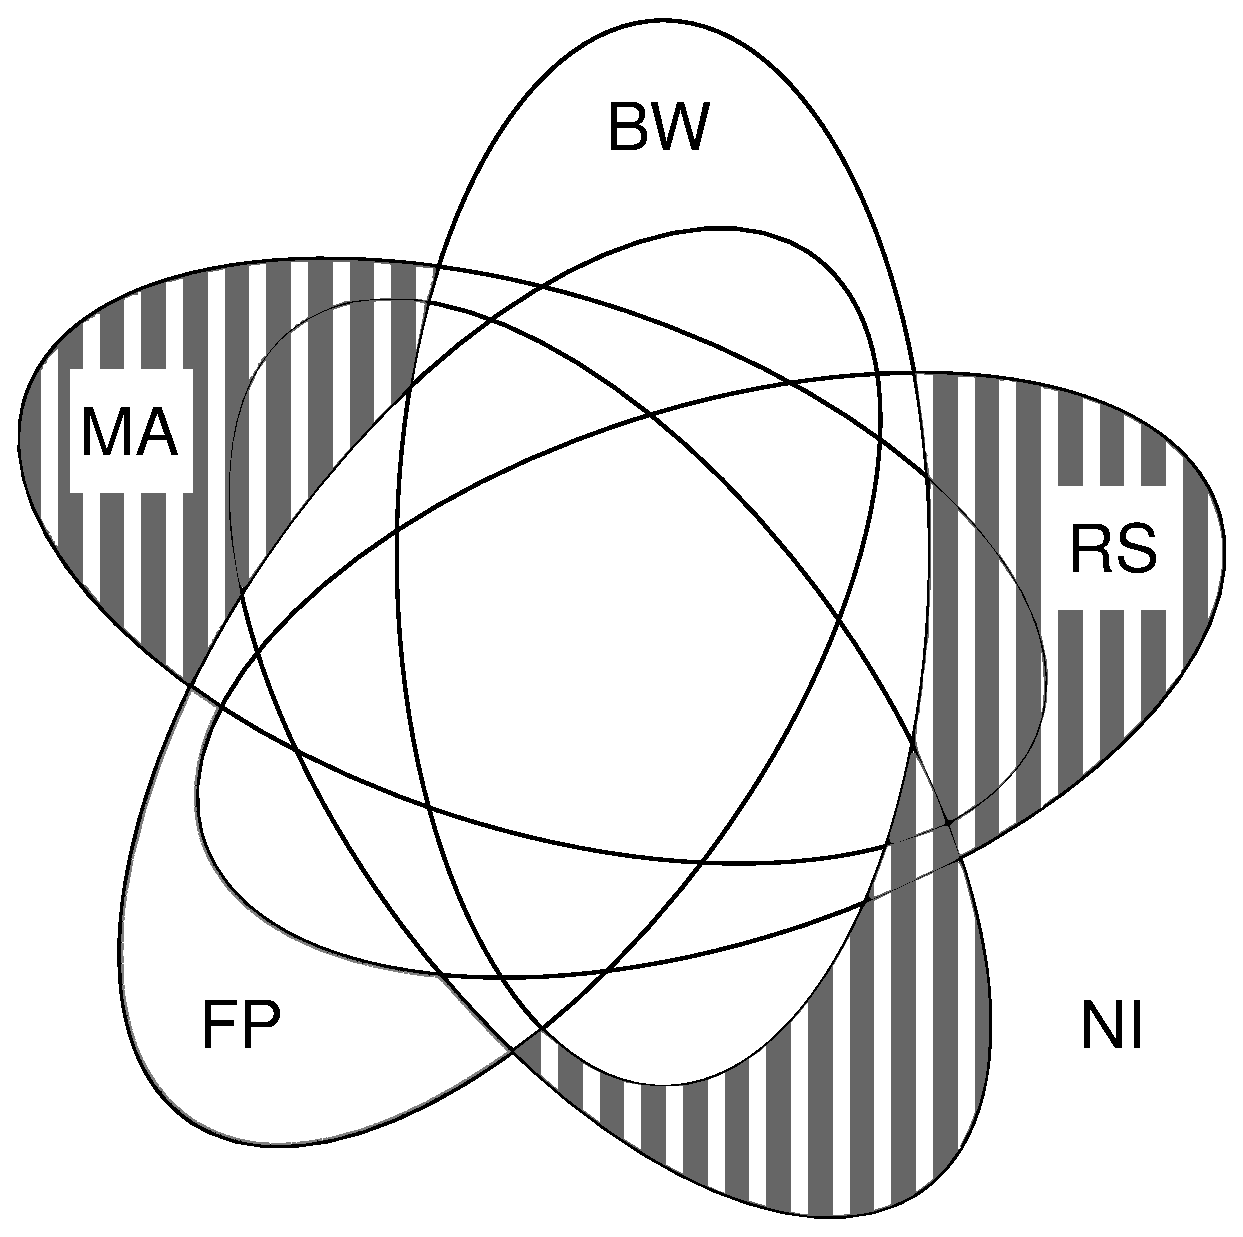
\includegraphics[width=0.48\columnwidth]{figs/venn_matching.pdf}
\caption{Problem variants which can be solved using our matching approach.}
\label{fig:venn_match}
\end{wrapfigure}
\end{comment}


\subsection{Dynamic Programming ($\FP+\CC+\MA+\BW$)}\label{ssec:dyn}

We now show that also the $\FP+\CC+\MA+\BW$ problem variant can be solved
in polynomial time. Note that this problem variant is non-trivial,
and that collocating nodes with chunks (i.e., embedding virtual machines
at the servers hosting the chunks) can be bad.

\stefan{carlos figure comes here}

%\maciek{TODO: In each of previous sections we had an example where we show
%  non-triviality of the problem. Here we also have an interesting
%  example, which show that placing VMs on chunks can be arbitrarily
%  bad. In this example optimal solution places each VM in separate
%  subtree and transports every chunk to this subtree. The subtree was
%  chosen because it was able to host all the machines, unlike the
%  subtries with chunks. The reader might wonder why we considered
%  every possible location for a VM and this is exactly the reason}

Our proposed approach is based on dynamic programming, and
leverages the \emph{optimal substructure property} of $\FP+\CC+\MA+\BW$:
as we will see, optimal solutions for subproblems (namely subtrees)
can efficiently be combined into optimal solutions for larger problems.
Indeed, the $\FP+\CC+\MA+\BW$ problem
exhibits such a structure, and we show how to exploit it to
compute efficient embeddings, even in scenarios where multiple chunks
need to be assigned to flexibly placeable nodes.

\textbf{Basic ideas.} For ease of presentation, we will transform the substrate network $\Tree$
into a binary tree, using binarization:
we clone every higher-degree node,
iteratively attaching additional clones as right children
and original children as left descendants.
%Last child is placed as
%right son of last clone.

As usual in dynamic programs, we define, over the structure of the tree, an inductive formula $f$ for
the minimal cost solution \emph{given} any possible number of virtual
machines embedded in a given subtree. (The actual set does not matter,
due to symmetry arguments.)
Our approach is to evaluate this function in a bottom-up
manner.
To finally compute the actual optimal embedding,
we traverse the computed minimal-cost path backwards.

Concretely, the first argument to function $f$
is a subtree $\Tree'$ (which contains a given set of chunks-in-the-subtree $\ChunkCount(\Tree')$),
and the
second argument is the number of nodes to be embedded in the subtree.
Function $f$ is evaluated in a bottom up manner. We initialize the
function at each leaf $\ell$, by $f(T_{\ell},x) =
\infty$ for all numbers of virtual machines $x$ which are larger than
the server capacity $\capacity(\ell)$;
to calculate $f(T_{\ell}, x)$, for $x \leq \capacity(\ell)$, we compute the
bandwidth allocation on the uplink of $T_{\ell}$, referred to by the function
$bw(T_{\ell},x)$: $bw(T_l,x)=  \CostTrans \cdot |x - |\ChunkCount(T_{\ell})||$ $
+ \CostCom \cdot (\Vms - x) \cdot x$,
which accounts for the bandwidth allocation on the uplink of $T_{\ell}$. The first
term represents the required bandwidth for the communication between the $x$
nodes on $\ell$, and the $\Vms - x$ nodes in the remaining parts of the substrate
network. 
%Obviously the communication $x$ among the $x$ nodes within $T_l$
%does not require bandwidth on the uplink of $T_l$. 
The second term represents
the bandwidth, which is necessary to transport the chunks from their location to
the node which should process the data (see Lemma~\ref{lemma:uplink} for more
details). 
%Since placing nodes on servers will not require additional bandwidth
%allocations, $bw$ is equal to $f$ on all subtrees $T_l$, which consist only of
%a single leaf. If the required bandwidth $bw$ exceeds the avialble bandwidth
%$\capacity$ on the uplink, $f(T_l,x)$ is set to $\infty$, to mark the
%corresponding number of nodes in the subtree as infeasible.}

%\carlo{
After this initialization, we proceed to compute $f$ for non-leaf
nodes in a bottom up manner: We consider every possible split of the $x$ nodes
into two positive integer
values: we put $r$ on the right and $x - r$ on the left subtree. 
That is, we take the optimal cost
(given recursively) of placing $r$ nodes in
the right subtree $\textsc{Ri}(T')$ of $T'$ and $x-r$ nodes in left subtree $\textsc{Le}(T')$ of
$T'$. Given the cheapest combination, we add the bandwidth requirements
on the uplink of $T'$ to generate the overall costs for placing $x$ virtual
machines in $T'$.
$$f(T',x) =   \min_{r \in \{0, \ldots, x\}}  f(\textsc{Ri}(T'), r) +
f(\textsc{Le}(T'), x - r) + bw(T',x)$$
Again, we set $f(T',x)$ to infinity if the required bandwidth
$bw$ exceeds the capacity $\capacity$ of the uplink of $T'$.

This allocation consists of two parts: (1) The node inter-connect
communication is easy to compute, as we know how many
virtual machines are in the left and right subtree, and how many are
outside.
%Concretely, for each node pair communicating across subtrees we
%charge $b_2 \cdot (w(e_1) +
%w(e_2))$, for each pair where one is in the subtree and the other outside,
%we charge $b_2 \cdot
%w(e_1)$. Right subtree case is symmetrical.
(2) The chunk access cost
can be computed by greedily matching nodes to chunks locally (first
inside the subtree, then across subtrees, then outside $T'$).
%In particular, we can
%just consider the absolute value of the difference between the number of chunks and
%the number of nodes in a given subtree, without knowing which
%is bigger, because in our model if there are some virtual machines
%left, we know that some chunks from outside will use the same transfer
%as if we have excessive chunks in the subtree.

%Assume there are $c_{\ell}$ chunks in the left and $c_r$
%chunks in the right subtree. To incline minimal cost we connect chunks in
%given subtree to virtual machines in the same subtree. If we can no
%longer do that, because $v_i < c_i (i \in \{l,r\})$, then we connect
%leftover chunks to virtual machines in second subtree of $T$. If we
%can no longer do that, we connect leftover chunks outside of $T$. This
%strategy is optimal, because connecting any other way can be amended
%(TODO: need better argument here), inclining lower cost. Connections
%inside either left or right subtrees inclines cost $0$ to edges $e_1$
%and $e_2$. Connections between left and right subtree incline cost
%$b_1
%\cdot (w(e_1) + w(e_2))$. Connections from either subtree to outside
%of $T$ inclines either $b_1 \cdot w(e_1)$ or $b_2 \cdot
%w(e_2)$. Finally, we can write down our formula for $f$:


%\maciek{We will want to go through all VM placements, for each of those do greedy matching and choose the cheapest.}%
%
%\maciek{Solution for subtree - how it can look like? It is ``partial matching''. Some matched VMs and chunks, but also some chunks transported out of subtree or some %VMs/slots that will have chunks transported into from outside. So we charge already those incomplete matchings.}

%\maciek{TODO: base cases for f that take into consideration hosting
%  multiple VMs in one node}%
%
%Therefore, we have:
%\begin{eqnarray*}
%f(T', x) &=& \min_{\ell \in \{0, \ldots, x\}}  f(\textsc{Le}(T'), {\ell}) + f(\textsc{Ri}(T'), x - {\ell}) \\
%&&+ \CostTrans(\textsc{Le}(T'),{\ell},\textsc{Ri}(T'),x-l)\\ &&+ \CostCom({\ell},x-{\ell})\\
%\end{eqnarray*}
%
%\maciek{We forgot to mention how we deal with bandwidth here. Our
%  approach is to check at every placement, at every subtree whether
%  uplink edge does not exceed its capacity. If it does for any subtree, we cross out
%  this placement. We also need to show correctness of this strategy in
%  analysis - but it holds from uplink lemma.}

\begin{comment}


\newcommand{\SumIndex}{\ensuremath{n}}
\begin{algorithm}[tbhp]
\DontPrintSemicolon % Some LaTeX compilers require you to use
%%\dontprintsemicolon instead
\SetAlgoNoEnd
\KwIn{$\Opt_{\SubstrateNode_l} ,
\Opt_{\SubstrateNode_r},
\ChunkCount_{\SubstrateNode_l},\ChunkCount_{\SubstrateNode_r} $}
$\ChunkCount_\SubstrateNode = \ChunkCount_{\SubstrateNode_l} +
\ChunkCount_{\SubstrateNode_r}$\;
\For{$\SumIndex \in \{0,\dots,\Vms\}$}{
  \For{$i \in \{0,\dots,\SumIndex\}$}{ \If{$\Opt_\SubstrateNode[\SumIndex]
  > \Opt_{\SubstrateNode_l}[i] +
\Opt_{\SubstrateNode_r}[\SumIndex - i]$}{
	$\Opt_\SubstrateNode[\SumIndex] \gets \Opt_{\SubstrateNode_l}[i]
	+
\Opt_{\SubstrateNode_r}[\SumIndex - i]$\;
    } }

 $bw \gets (\Vms -
\SumIndex) \cdot \SumIndex \cdot \CostCom +   |i -
\ChunkCount_\SubstrateNode| \cdot \CostTrans$\;
  \eIf{$bw \leq \capacity(\Uplink(v))$}{
    $\Opt_\SubstrateNode[\SumIndex] \gets \Opt_\SubstrateNode[\SumIndex]
    + bw$\; }{ $\Opt_\SubstrateNode[\SumIndex] \gets \infty$\; } }
%
\caption{$aggregate(\SubstrateNode \in \SubstrateNodes)$}
\label{algo:dynAggregation}
\end{algorithm}

List all needed functions like distance, counter of number of chunks
in subtree.

Tell how to go back through the array to reconstruct the actual
placements. Following path of minimas. Other approach is to store pointers to minimas on lower levels as those are chosen.

(Base case) We fill the entire array $Opt_l$ for the leaf $l$ with zeros. It means that we allow hosting $0, 1, \ldots, n$ VMs in this leaf. We can restrict the number of VMs that are hosted in the same leaf by some constant $x$ (that can be independent for every leaf) by setting $Opt_l[x+1] = Opt_l[x+2] = \ldots = Opt_l[n] = \infty$.

\end{comment}


\textbf{Analysis.}
The correctness and optimality of our dynamic program
is due to the decoupling of the costs induced by the tree
structure of $\Tree$ and the  substructure
optimality property.
The substructure optimality follows from the observation that
costs can be accounted on the uplink, and the fact
 that we check each possible node distribution.
For each substrate vertex ($n_S$ many) we have
to check the cost of all possible splits,
resulting in an overall complexity of $\mathcal{O}(n_S \cdot n_V)$.
(The runtime to binarize $\Tree$ is asymptotically negligible.)

%\textbf{Summary.}
%Figure~\ref{fig:venn_dp} summarizes all problem
%variants which can be solved with our dynamic programming approach.
%\begin{wrapfigure}{r}{0.5\columnwidth}
%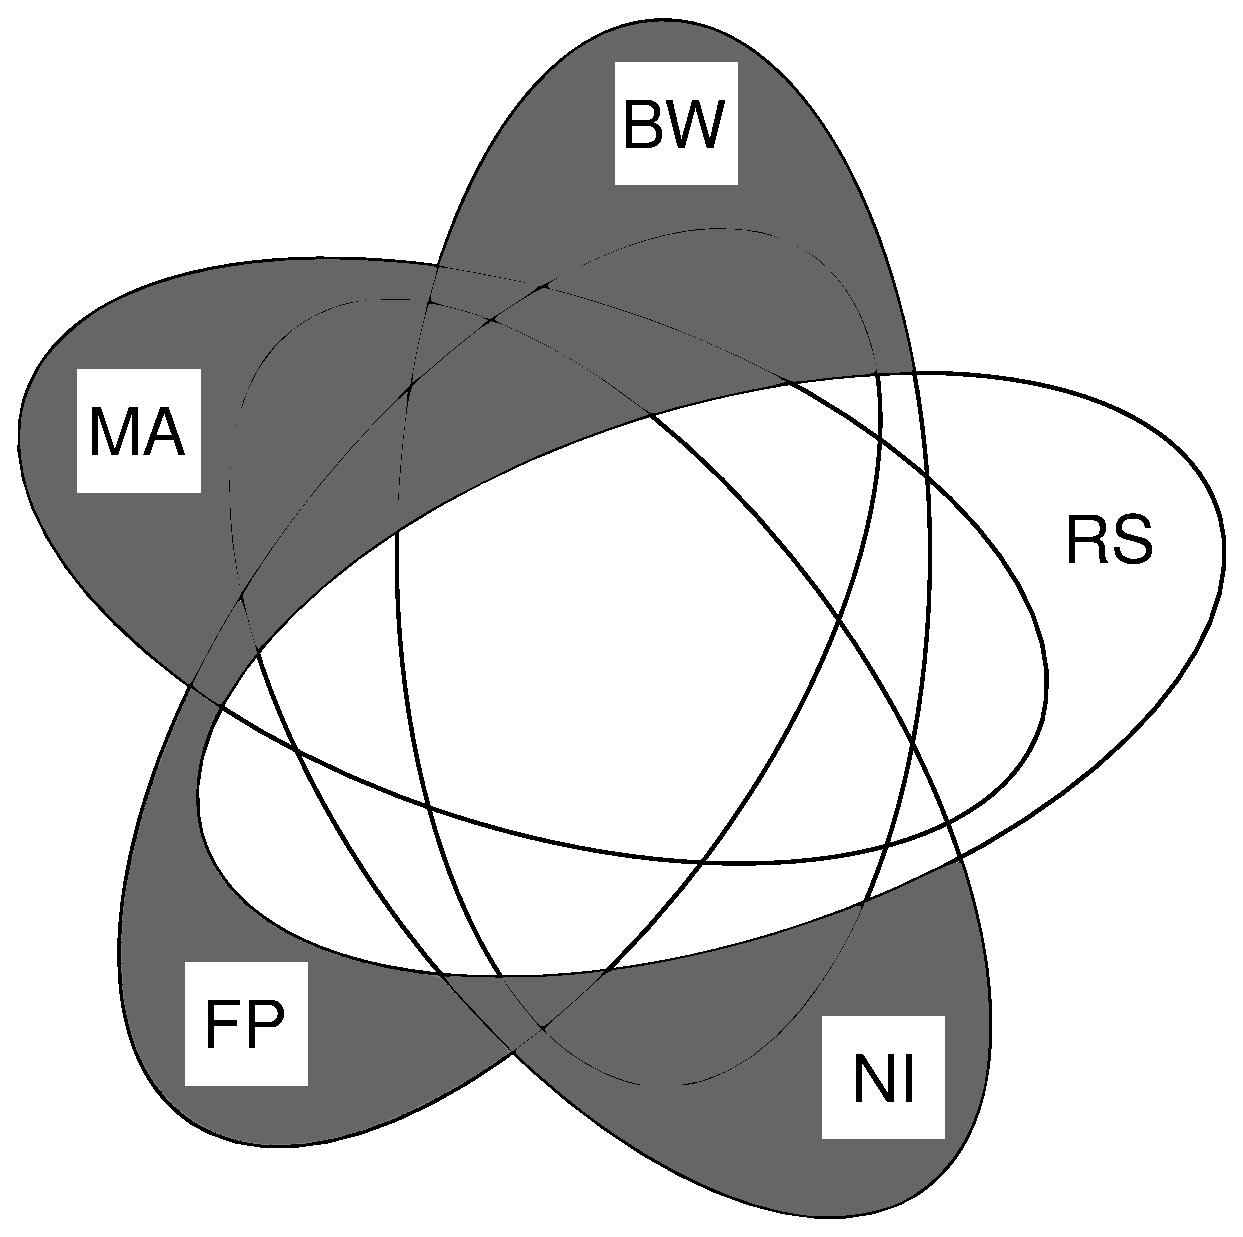
\includegraphics[width=0.48\columnwidth]{figs/venn_dp.pdf}
%\caption{Variants solved by programming approach.}
%\label{fig:venn_dp}
%\end{wrapfigure}

\subsection{Remark: Simple Problems}

To conclude, for the sake of completeness, we also observe that there are
several problems which
allow for a trivial solution. Concretely, problems with $\FP$
plus any combination of
$\RS$ and $\BW$ (but without $\CC$ or $\MA$) can easily be solved by mapping nodes to chunk locations.
Figure~\ref{fig:venn_trivial}
shows a Venn diagram of the trivial property combinations.

\begin{wrapfigure}{r}{0.5\columnwidth}
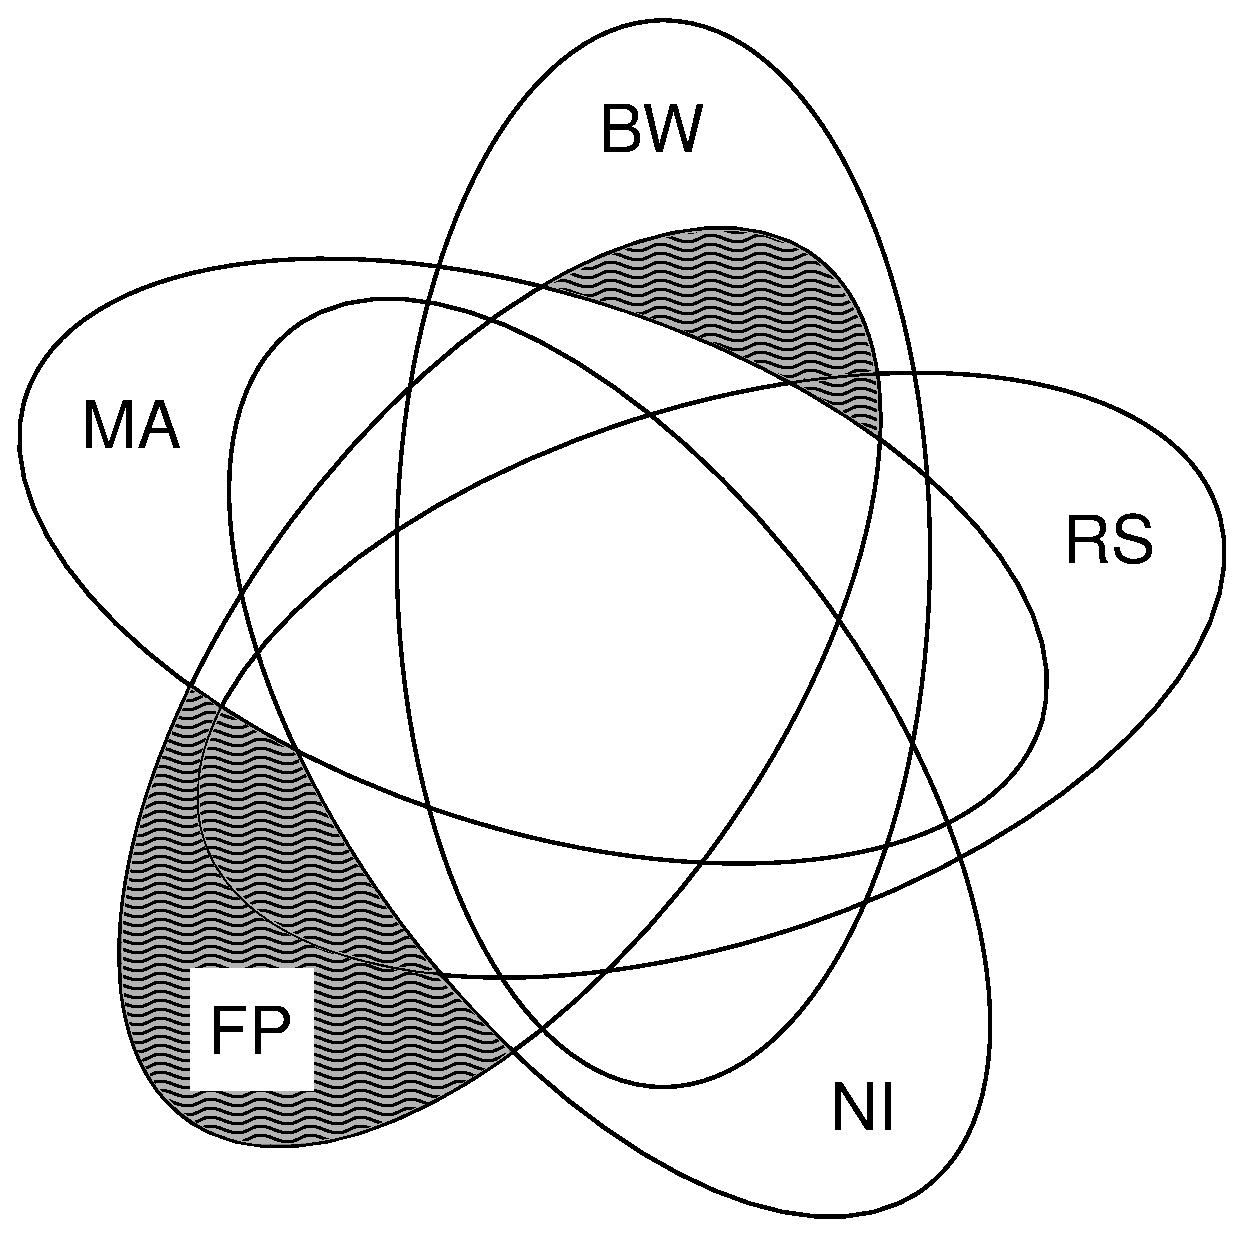
\includegraphics[width=0.48\columnwidth]{figs/venn_trivial.pdf}
\caption{Trivially solvable problem variants.}
\label{fig:venn_trivial}
\end{wrapfigure}


%%%%%%%%%%%%%%%%%%%%%%%%%%%%%%%%%%%%%
\section{NP-Hardness Results}\label{sec:np}

%\carlo{TODO: Move embedd in surrounding text / move. Figure~\ref{fig:venn_full}
%gives an overview of the problems, which have been solved in polynomial time in
%Section~\ref{sec:poly}. This section will present proofs to show that all
%remaining property combinations (marked in black) are np-hard.}

We have seen that even problems with multiple dimensions of
flexibility can be solved optimally in polynomial time.
This section now points out fundamental
limitations in terms of computational tractability. In particular, we
will show that problems become NP-hard if multiple replicas have to be
assigned to a flexibly placeable node ($\FP+\RS+\MA$ is proved NP-hard in
Section~\ref{ssec:fprsma}), and if inter-connects have to be established
between flexible nodes ($\FP+\RS+\CC$ is proved NP-hard in Section~\ref{ssec:fprscc}); both
results hold even in uncapacitated networks, and even in small-diameter
substrate networks (namely two- or three-level trees~\cite{fattree}).
The hardness of $\FP+\RS+\MA$ and $\FP+\RS+\CC$ imply
the hardness of four additional, more general models, as
summarized in the following figure:

\begin{figure}[htbp]
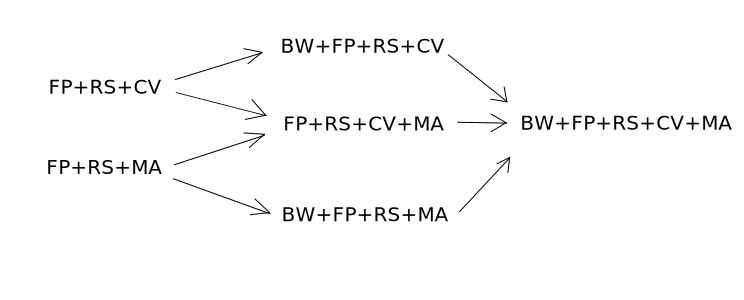
\includegraphics[width = \columnwidth]{figs/np-hierarchy}
\end{figure}


\subsection{Introduction to 3D Perfect Matching}

Both the hardness of $\FP+\RS+\MA$ and $\FP+\RS+\CC$ is shown by a reduction
from the NP-complete problem of \emph{3D Perfect Matching}~\cite{3dmatch},
which
can be seen as a generalization of bipartite matchings to 3-uniform
hypergraphs. We will refer to this problem by $\TDM$, and for completeness,
review it in the following.

$\TDM$ is defined as follows. We are given three finite and disjoint
sets $X$, $Y$, and $Z$ of cardinality $k$, as well as a subset of triples $T\subset
X \times Y \times Z$.  Set $M \subseteq T$ is a 3-dimensional matching
if and only if, for any two distinct triples $t_1=(x_1, y_1, z_1) \in M$
and $t_2=(x_2, y_2, z_2) \in M$, it holds that $x_1\neq x_2$, $y_1\neq
y_2$, and $z_1\neq z_2$. Our goal is to decide if we can construct
a $M \subseteq T$ which is \emph{perfect}, that is, a subset which covers all
elements of $X \times Y \times Z$.

%TODO: image like this: \url{https://upload.wikimedia.org/wikipedia/commons/thumb/5/50/3-dimensional-matching.svg/240px-3-dimensional-matching.svg.png}

\subsection{Multi-Assignments are hard ($\FP+\RS+\MA$)}\label{ssec:fprsma}

Our proof that $\FP+\RS+\MA$ is NP-hard is based on the following main ideas.
We encode an $\TDM$ instance as an $\FP+\RS+\MA$ instance as follows:

 \begin{itemize}
 \item For every element in the universe $X\cup Y\cup
 Z$, we create a chunk type. Intuitively, in $\TDM$,
 each element must be covered, which corresponds to the requirement
 of $\FP+\RS+\MA$,
 that each chunk type is processed.

 \item We will encode each triple as three leaves in
 a substrate tree $\Tree$. The three leaves are close to each
 other in $\Tree$, and the placement of chunk replicas in $\FP+\RS+\MA$
 corresponds to the elements of the
 triples in these leaves.

 \item The node placement will correspond to choice of triples,
 independently in which leaf the node is mapped.
 A node will process the chunk which is located on the same server,
 as well as the chunks in other two leaves of the same gadget.

\item We will use threshold $\Thr$  to ensure that no node
will process
any chunk outside its gadget.
\end{itemize}

\textbf{Construction.}
Given an instance $I$ of $\TDM$, we construct an instance $I'$ of
$\FP+\RS+\MA$ as follows:
\begin{itemize}
\item \emph{Tree Construction:} We create a tree consisting of a root,
and for each triple, we create a gadget which we directly attach as
child of the root. The gadget is of height 2,
and has the following form:
The gadget of each triple $t_i$ consists of an inner node (a router) and three leaves.
\item \emph{Chunks and chunk replicas:} For each element in $X$, $Y$ and $Z$,
 we create a chunk type
($3 \cdot k$ in total). Every gadget
contains three chunk replicas, corresponding to the elements of $t_i$.
\item \emph{Other properties:} We set the number of to-be-embedded nodes to $k$,
$\CostTrans$ to $1$, and the number of slots in each node to $m=3$ \stefan{what
is the number of slots here?}\maciek{it is number of replicas that
each VM can process (the MA property)}. We use a threshold $\Thr=2 \cdot 2
\cdot k$. \maciek{If we update the model to take care of hosting
  multiple VMs in one leaf, we should set this instance to allow only
  one VM per leaf. However, any number of VMs per leaf will be OK for
  this proof.}
\end{itemize}

The construction is illustrated in Figure~\ref{fig:fprsma}.
%\begin{figure}[htbp]
%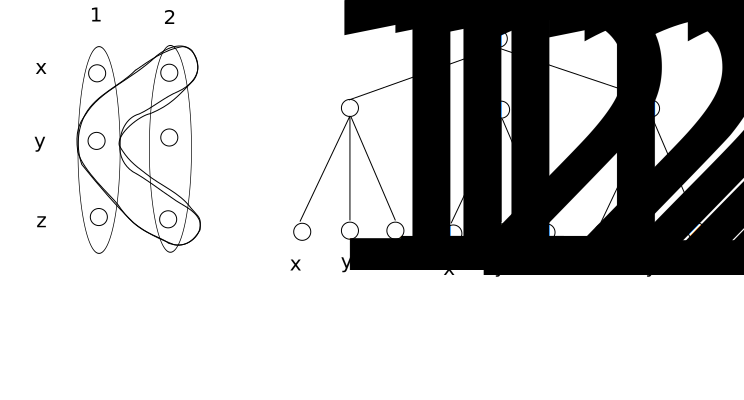
\includegraphics[width = \columnwidth]{figs/example-matching}
%\end{figure}
\begin{figure}[htbp]
\includegraphics[width = 0.3\columnwidth]{figs/np_3dm_formular}
\hfill
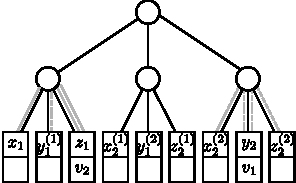
\includegraphics[width = 0.6\columnwidth]{figs/np_3dm_construction}
\caption{\textit{(Left:)} A $\TDM$ instance with three triples:
$(x_1, y_1, z_1)$, $(x_2, y_1, z_2)$, and $(x_2, y_2, z_2)$. The solution is
indicated by the grey triples; the dashed triple is not used for the
solution. \textit{(Right:)} The corresponding problem and solution of $\FP + \MA
+ \RS$.}
\label{fig:fprsma}
\end{figure}
\stefan{TODO: finish picture and add a caption explaining its
elements}


\textbf{Correctness.}
Given these concepts, we can now show the computational hardness.
\begin{theorem}
$\FP+\RS+\MA$ is NP-hard.
\end{theorem}
\begin{proof}
Let $I$ be an instance of $\TDM$ and let $I'$ be an instance of
$\FP+\RS+\MA$ constructed as described above.
We prove that $I'$ has solution of cost $\leq \Thr$ if ($\Rightarrow$) and only if
($\Leftarrow$)
$I$ has a matching of size $k$.

($\Rightarrow$) Let us take a solution to $\TDM$. We place a node in every
gadget that corresponds to the chosen triples. We match every chunk in a
gadget to a node in this gadget (only the chosen ones). This solution has
cost exactly $\Thr$. As every element of the universe is covered, every
chunk type is processed.

($\Leftarrow$) Let us take a solution to $\FP+\RS+\MA$ of cost $\leq \Thr$. We
choose triples that correspond to gadgets where there are nodes. Since
all chunks are processed, very element of $X$, $Y$ and $Z$ is matched. Each
node must processes chunks that correspond to the triple, otherwise the
cost must be larger than $\Thr$ (high costs for the connection between
nodes and chunks).
\end{proof}


\subsection{Inter-connects are hard ($\FP+\RS+\CC$)}\label{ssec:fprscc}

Next, we prove that the joint optimization of node placement and replica selection
is NP-hard if an inter-connect has to be established between virtual machines.
In our terminology, this is the $\FP+\RS+\CC$ problem.

\textbf{Construction.}
Let $I$ be an instance of $\TDM$. We will create an instance $I'$
for $\FP+\RS+\CC$ as follows:
\begin{itemize}
\item We will construct the same tree as in previous reduction with
chunk replicas placed in the same way.
\item The communication cost in the inter-connect is set to $\CostCom = 1$.
\item The number of nodes (virtual machines) is $\Vms = 3 \cdot k$.
\item We use a threshold $\Thr =  6 \cdot k + 3 \cdot 3 \cdot 2 \cdot
(k - 1) \cdot k$.  \maciek{If we update the model to take care of hosting
  multiple VMs in one leaf, we should set this instance to allow only
  one VM per leaf. In this proof it also does not matter, as it is
  already forced by infinite transportation cost, however we need to
  define it anyway.
  }
\item We set the access cost $\CostTrans$ to a chunk replica to a high value $W$. This will force
nodes to be collocated with the replica. One example of sufficient
(and polynomial) $W$
is the value of threshold, defined above. \maciek{it is not minimal,
  but clean and sufficient}
\end{itemize}


\textbf{Proof of correctness.}
Intuitively, in order to minimize embedding costs,
nodes should be placed on near-by replicas. We use the following
helper lemma.
\begin{lemma}\label{lemma:helper}
In every valid solution of $I'$ of cost $\leq \Thr$, each gadget
falls in one of two categories:
$k$ gadgets have exactly
$3$ nodes, and $n-k$ gadgets remain empty.
\end{lemma}
\begin{proof}
Since $W=\infty$, nodes will always be placed
directly on chunks (the access network cost is zero).
Moreover, since
is valid, $3 \cdot k$ nodes are mapped
directly to the different chunk locations.
Now, consider any pair of nodes communicating over the
inter-connect; due to our construction, the communication cost
for each such pair is either
2 hops (if they belong to the same gadget) or 4 hops (if they belong
to different gadgets).
The lemma then follows from the observation that $\Thr$
is chosen such that it is never possible to distribute nodes
among more than $k$ gadgets.
\end{proof}

\begin{theorem}
$\FP+\RS+\CC$ is NP-hard.
\end{theorem}
\begin{proof}
Let $I$ be an instance of $\TDM$ and let $I'$ be an instance of
$\FP+\RS+\CC$ constructed as described above.
We prove that $I'$ has solution of cost $\leq \Thr$ if ($\Rightarrow$) and only if
($\Leftarrow$)
$I$ has a solution.

($\Rightarrow$) In order to compute a solution
for $I'$ given a solution for $I$, we proceed as follows.
Given a covering set of triples $S = \{t_1, t_2, \ldots, t_k\}$, we place three nodes in each gadget that
corresponds to every triple of $S$. Chunks are matched to nodes that are located
on the same server.

The solution has the following cost:
(1) the communication cost inside a gadget is $2 \cdot {3 \choose 2}$,
  as every pair contributes two hops;
  (2) the communication cost from each gadget to all other gadgets is $4
  \cdot 3 \cdot 3 \cdot (k - 1) / 2$, where the factor $4$ is
  for the
  communication over $4$ hops, the factor $3$
  corresponds to the number of nodes per gadget, and
  $3 \cdot (k-1)$ is the number of nodes in remote gadgets;
  as we count each pair twice, we need to divide by two in the end.
Summing up over all $k$ gadgets, we get exactly $\Thr$.

($\Leftarrow$) Given a solution for $I'$,
we can exploit Lemma~\ref{lemma:helper} to construct a solution for $I$.
We know that in any solution of cost at most $\Thr$,
$k$ gadgets contain exactly 3 nodes. These gadgets correspond to a valid
3D Perfect Matching: every
chunk was processed and hence every element in the $X \cup Y \cup Z$ is covered.
\end{proof}


%%%%%%%%%%%%%%%%%%%%%%%%%%%%%%%%%%%%%
\section{Related Work}\label{sec:relwork}

There has recently been much interest in programming models and distributed
system architectures for the processing and analysis of big data (e.g.~\cite{nodb,mapreduce,shark}). The model studied in
this paper is motivated by MapReduce~\cite{mapreduce} like batch-processing applications, also known
from the popular open-source implementation \emph{Apache Hadoop}.
These applications
generate large amounts of network traffic~\cite{orchestra,talk-about,amazonbw},
and over the last years, several systems have been proposed which provide
a provable network performance, also in shared cloud environments, by supporting explicit
relative~\cite{faircloud,elasticswitch,seawall}
or, as in the case of our paper, \emph{absolute}~\cite{oktopus,secondnet,drl,gatekeeper,proteus} bandwidth reservations
between the virtual machines.
In particular, the notion of virtual networks which combine compute and network resources has been introduced.
For a good survey on network virtualization and in particular virtual network embeddings,
we refer the reader to~\cite{boutaba-survey} and~\cite{fischer-survey}.

The most popular virtual network abstraction for batch-processing applications today is the \emph{virtual cluster},
introduced in the Oktopus paper~\cite{oktopus}, and later studied by many others~\cite{talk-about,proteus}.
Several heuristics have been developed to compute ``good'' embeddings of virtual clusters: embeddings
with small footprints (minimal bandwidth reservation costs).~\cite{oktopus,talk-about,proteus}
The virtual network embedding problem has also been studied for more general graph abstractions
(e.g., motivated by wide-area networks).~\cite{infocom2009,ammar,turner,simannealing,ucc12mip,zhu06}

From a theoretical perspective, the virtual network embedding problem can be seen as a generalization
of classic VPN graph embedding problems~\cite{Goyal2008,gupta2001provisioning},
in the sense that in virtual network embedding problems, also the embedding endpoints are flexible and subject to optimization.
In this sense, the virtual network embedding problem can also be seen as a generalization of the
classic NP-hard Minimum Linear Arrangement problem which asks for the
embedding of guest graphs on a simple \emph{line topology} (rather than tree-like topologies as
studied in this paper).~\cite{mla,mla-survey}
There exist several interesting algorithms for the Minimum Linear Arrangement problem,
e.g., providing sublogarithmic approximation ratios~\cite{mla-feige}.

However, to the best of our knowledge, we are the first to provide an algorithmic
study of the virtual cluster embedding problem which takes into account
data locality as well as the possibility to select replicas. As we have shown in this paper,
the resulting problems can be seen as interesting new variants of several classic optimization
problems, such as hitting set and 3-dimensional matching problems~\cite{3SC-hard} as well as flow problems~\cite{korte2002combinatorial}.

%%%%%%%%%%%%%%%%%%%%%%%%%%%%%%%%%%%%%
\section{Summary and Conclusion}\label{sec:conclusion}

This paper investigated data data locality aware algorithms which exploit two fundamental
degrees of freedom in virtual cluster
embedding problems: replica selection and flexible node placement. In order to
chart the landscape of the problem complexity, we
decomposed the problem into its fundamental aspects,
namely $\RS$, $\MA$, $\FP$, $\CC$, and $\BW$, and studied the computational
tractability of different combinations.

In particular, we have shown that
at the heart of our model lie interesting new variants of classic
optimization problems related to matchings and flows. Interestingly, despite the
different dimensions of flexibility (in terms of replica selection, assignment and embedding),
many problem instances can actually be solved in polynomial time.
On the negative side, we have also shown that there exist computationally hard
problems even in uncapacitated networks. In particular,
we have shown that several embeddings problems are NP-hard already in two- and three-level trees
(a practically relevant result given today's datacenter topologies~\cite{fattree}),
and even if the the number of replicas is bounded by two.

\begin{table}


\begin{small}
\begin{tabular}{|l|l|p{4cm}|}
\hline
\multirow{3}{*}{NP-hard} & 5 combinations & \mbox{$\RS+\MA+\FP+\CC+\BW$}\\
\cline{2-3}
 & 4 combinations &  \mbox{$\RS+\MA+\FP+\CC$}; \mbox{$\RS+\MA+\FP+\BW$};
\mbox{$\RS+\FP+\CC+\BW$} \\ \cline{2-3}
 & 3 combinations &\mbox{$\RS+\MA+\FP$};\mbox{$\RS+\FP+\CC$} \\
 \hline
 \hline
\multirow{3}{*}{Flow} & 4 combinations & \mbox{$\RS+\MA+\CC+\BW$} \\ \cline{2-3}
 & 3 combinations & \mbox{$\RS+\CC+\BW$};\mbox{$\RS+\MA+\BW$}    \\ \cline{2-3}
 & 2 combinations &$\RS+\BW$ \\
 \hline
 \hline
\multirow{3}{*}{DP} & 4 combinations & \mbox{$\MA+\FP+\CC+\BW$} \\ \cline{2-3}
 & 3 combinations &   \mbox{$\MA+\FP+\CC$};
\mbox{$\MA+\FP+\BW$}; \mbox{$\FP+\CC+\BW$} \\ \cline{2-3}
 & 2 combinations &\mbox{$\MA+\FP$}; \mbox{$\FP+\CC$};
\mbox{$\FP+\BW$} \\
 \hline
 \hline
\multirow{3}{*}{Matching} &3 combinations&
\mbox{$\RS+\MA+\CC$};\mbox{$\MA+\CC+\BW$}  \\
\cline{2-3}
 & 2 combinations & \mbox{$\RS+\MA$};
\mbox{$\RS+\CC$}; \mbox{$\MA+\CC$};
\mbox{$\MA+\BW$};\mbox{$\CC+\BW$} \\ \cline{2-3}
& 1 combinations & \mbox{$\RS$}; \mbox{$\MA$};
\mbox{$\CC$};\mbox{$\BW$}\\
 \hline
 \hline
 \multirow{3}{*}{0 Cost} & 3 combinations & \mbox{$\RS+\FP+\BW$}\\
\cline{2-3}
 & 2 combinations & \mbox{$\RS+\FP$}; \mbox{$\FP+\BW$}
\\ \cline{2-3}
 & 1 combinations & \mbox{$\FP$}\\
 \hline
\end{tabular}
\end{small}
\caption{\maciek{This summary is wrong, I sent you an update in e-mail
  (original image summary.pdf is wrong as well - see update)}The use cases of the proposed algorithms, expressed in property
combinations which it can solve faster, than any other algorithm.}
\label{tab:summary}
\end{table}


Our results are summarized in
Figure~\ref{fig:summary}.
One interesting takeaway from this figure regards
the question which properties render the problem
NP-hard. For instance, we see that interestingly, $\BW$
does not influence the hardness of any problem variant,
while $\RS$ is crucial for NP-hardness.
$\MA$ only affects hardness if combined with $\RS$.
$\CC$ is trivial without $\FP$, and $\FP$ requires
more sophisticated algorithms when combined with $\CC$ or $\MA$;
in combination with $\RS$ and $\MA$ or $\CC$, $\FP$ renders the
problem NP-hard.

%\begin{figure}
%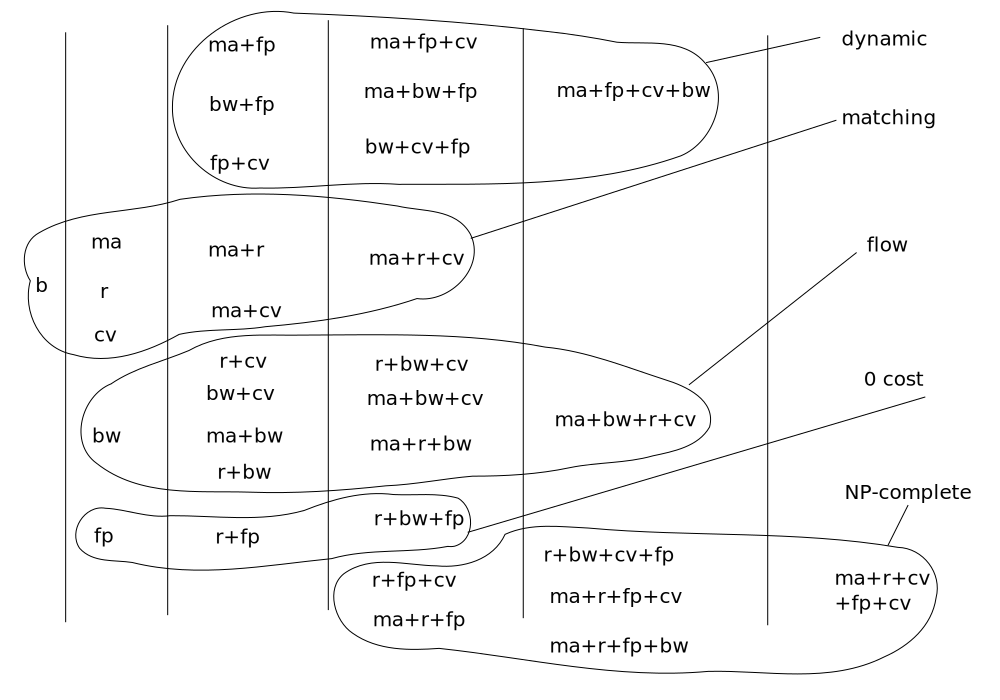
\includegraphics[width=\columnwidth]{figs/summary}
%\caption{\maciek{This figure is wrong in couple places, but I sent you an e-mail what should be redone.}Summary of results. As this paper only presented algorithms %(approaches indicated in the same
%color and pattern as in the previous figures) for the most
%difficult problems and, respectively, proved NP-hardness (indicated in black) of the simplest
%problems, several additional results are simple implications. In this figure,
%we always suggest the best (simplest and fastest) approach to solve a specific problem variant.}
%\label{fig:summary}
%\end{figure}


%\begin{figure}[t]
%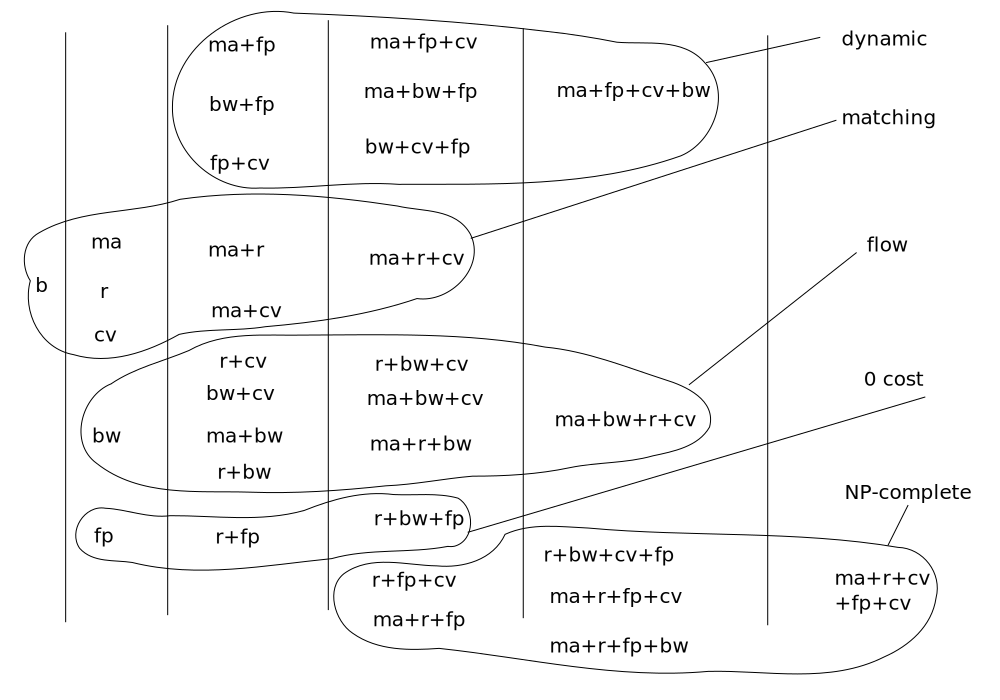
\includegraphics[width = \columnwidth]{figs/summary}
%\caption{Summary of results. As this paper only presented algorithms for the most
%difficult problems and, respectively, proved NP-hardness of the simplest
%problems, several additional results are simple implications (indicated by arrows).}
%\label{fig:summary}
%\end{figure}


Our paper draws an almost complete picture of what can and cannot be
computed optimally in our setting, and may be of interest both to the algorithm
and the networking community. At the same time, we understand our model and work
as a first step, and believe that our paper opens several interesting
questions for future research, for instance, regarding randomized
or approximation algorithms.


%%%%%%%%%%%%%%%%%%%%%%%%%%%%%%%%%%%%%
%\bibliographystyle{alpha}
\bibliographystyle{abbrv}
\bibliography{references}

%%%%%%%%%%%%%%%%%%%%%%%%%%%%%%%%%%%%%
\begin{appendix}

\section{The Bandwidth Lemma}

The following lemma is useful in our NP-hardness proofs.

\begin{lemma}[Bandwidth Lemma]\label{lem:bandwidth-lemma}
  Let $\clauses$ and $\variables > 4$ be two arbitrary positive integers. Let $a_1, a_2, \ldots,
  a_{\variables}$ be a sequence of $\variables$ integers which adds up to $\clauses \cdot \variables$. Also, for
  each $i$ we have $a_i \leq 2 \cdot \clauses$. Then it holds that if
  $$ \forall_i:~~ a_i \cdot (\clauses \cdot \variables - a_i) \leq \clauses \cdot (\clauses \cdot \variables -
  \clauses), $$
\noindent  then for each $i$: $a_i = \clauses$.
\end{lemma}
\begin{proof}
For the sake of contradiction, let us assume that there exists an index $k$ such that
$a_k \neq \clauses$. Then we can distinguish between two cases:
either $a_k<\clauses$ or
$a_k>\clauses$.

\textbf{Case $a_k<\clauses$:} If there exists a $k$ with $a_k<\clauses$,
due to the fact that the sequence adds up to $\clauses \cdot \variables$,
there must also exist a $k'$ such that $a_{k'}<\clauses$ (by a simple
pigeon hole principle). Thus, this case can
also be reduced to the second case (\textbf{Case $a_k>\clauses$}) proved
next.

\textbf{Case $a_k>\clauses$:} Since it also holds that $a_k < 2\clauses$,
$a_k$ must be of the form $\clauses + x$ for $x \in [1, \ldots, \clauses]$.
Let us consider the (bandwidth) inequality:
$$ (\clauses + x) \cdot (\clauses \cdot \variables - \clauses - x) \leq \clauses \cdot (\clauses \cdot \variables - x) $$

This can be transformed to:

$$ 0 \leq x(x - (\clauses \cdot (\variables - 2))) $$

The equation holds for $x \leq 0$ or $x \geq \clauses \cdot (\variables - 2)$,
and no
positive $x \leq \clauses$ can satisfy this inequality for $\variables > 4$. Contradiction.
\end{proof}


\section{Replica selection is hard}\label{ap:tworep}

\maciek{We need to introduce the idle machines extension, that is
  needed for reduction to work. Motivation: We can say that idle vms are only idle in
  mapping phase of MapReduce, but participate in shuffle phase. We can
  call it ``Additional shuffle nodes extension''.We can also tell the reader that our
  dynamic program works for this extension (f(T,x,idle)) . Considering
  mixing this extension with $\MA$:
   (1) NP-hardness
  proofs holds with setting $idle=0$; (2) dynamic program work with
  assumption that every VM either processes 0 chunks or processes
  maximum number of chunks (3) our flow algorithm
  work with contrary model assumption, that we can have arbitrary
  number of chunks assigned to VMs. }

We have seen that replica selection flexibilities can render problems computationally hard.
In the following, we will explore the minimal requirements for rendering replica selection hard.
In particular, we will show that already two replicas for each chunk type are sufficient to
introduce intractability.

\maciek{We need to tell the reader that our proof holds only for
  (NP-complete) subset of 3SAT where we have more than 4
  clauses. Otherwise the bandwidth lemma does not work!}


In the following, we first give an alternative proof for the hardness of $\CC+\FP+\RS+\BW$.
Subsequently, we show that the 2-replica variant $\RS(2)$ is hard.
For our proof, we assume a model where there can be more nodes than chunk types,
and additional nodes only participate in the inter-connect, and not the replica access network.

% TODO
%\subsection{Three replicas are hard ($\CC+\FP+\RS+\BW$)}\label{ssec:three}

We first prove that $\CC+\RS+\FP+\BW$ is NP-hard by reduction from the Boolean Satisfiability Problem ($\SAT$).
Since $\SAT$ is a decision
problem, we transform $\CC+\RS+\FP+\BW$ into a decision problem too, by
introducing a cost threshold $\Thr$.

Let's first recall that the $\SAT$ problem asks whether a positive valuation exists
for a formula $\Formula$ with $\clauses$ clauses and $\variables$ variables.
In the following, we will only focus on $\SAT$ instances of at least four variables;
this problem remains NP-hard.

\textbf{Construction.}
Given any formula $\Formula$ in Conjunctive Normal Form (CNF) with at least four variables, we produce
a $\RS+\FP+\BW$ instance as follows. First, we construct a substrate tree $\Tree_{\Formula}$, consisting of
a root and separate gadgets for each variable of $\Formula$, each of which
is a child of the root.
The gadget of variable $\variab$ has a root, $\aroot(\variab)$, and two children:
$\positive(\variab)$ and $\negative(\variab)$. Child $\positive(\variab)$ has $\clauses$
many children $\nu_1, \nu_2, \ldots, \nu_{\clauses}$, and child
$\negative(\variab)$ has
$\clauses$ many children $\neg \nu_1, \neg \nu_2, \dots, \nu_{\clauses}$. Every
gadget has the same structure: the same height and the same number of
leaves. This construction is illustrated in
Figure~\ref{fig:construction_3sat}.


\begin{figure}
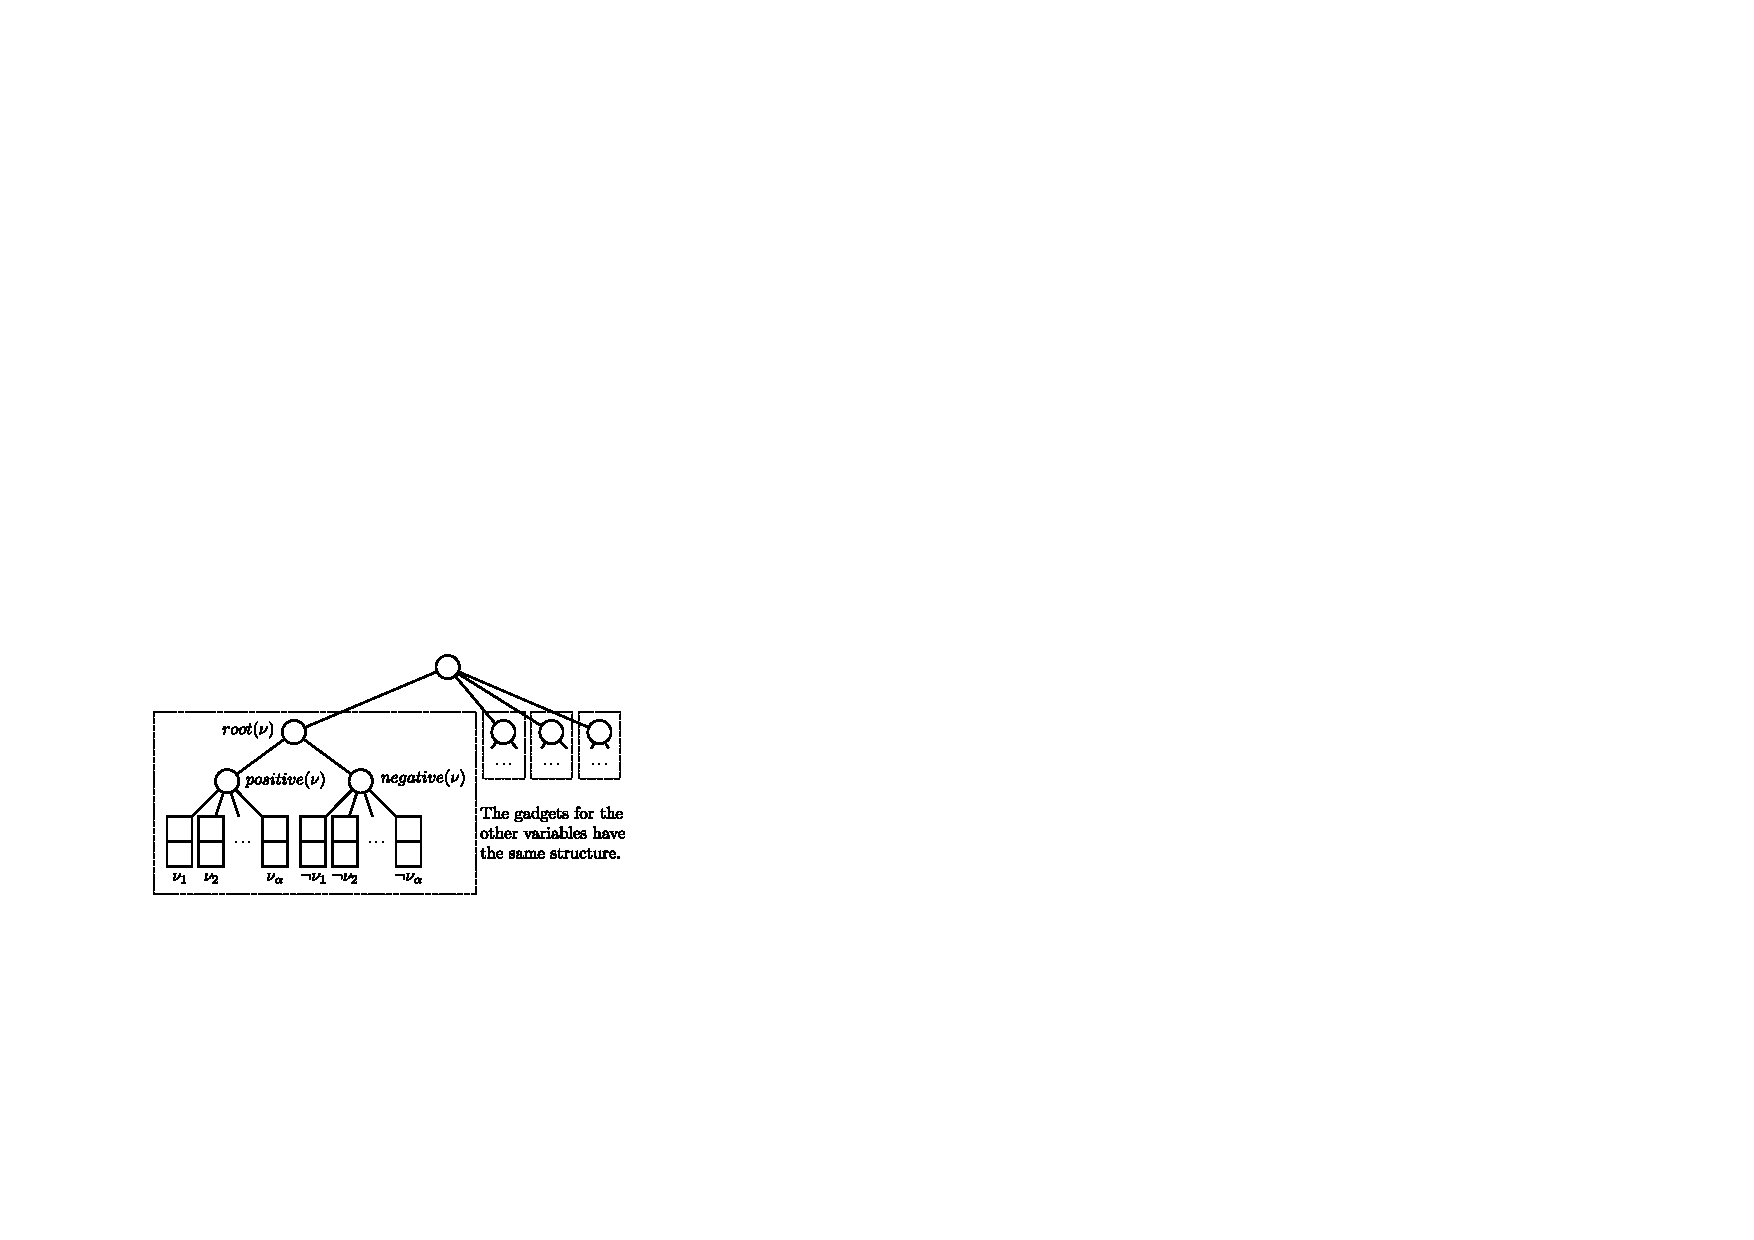
\includegraphics[width=\columnwidth]{figs/construction_3sat}
\caption{The construction of the gadget for $\nu$. If $\nu$ appears in the
first clause, a chunk $\achunk_1$, will be located at $\nu_1$. If $\neg \nu$
satisfies the last clause, $\neg
\nu_\alpha$ will host $\achunk_\alpha$.}
\label{fig:construction_3sat}
\end{figure}


By default, we will set the available
bandwidth to be the
same everywhere, in every gadget; differences will be shown when we
will place chunks.

We set the number of virtual machines to $\Vms = \clauses \cdot \variables$.
Moreover, we define the inter-connect communication cost to be $1$,
and the access cost to be a sufficiently large constant $W$,
such that nodes must always be collocated with chunks.
(For a concrete value, see Appendix~\ref{ap:W}).

We set the following bandwidth capacities in the substrate. There are three
levels of edges in the substrate network $\Tree_{\Formula}$ given by formula
$\Formula$: \emph{top}, \emph{middle} and \emph{bottom}.
We do not consider any capacities at the \emph{bottom} and \emph{middle} levels.
At a top-level edge, we set the bandwidth to $\clauses \cdot (\clauses
\cdot \variables -
\clauses)$.

We set the number of chunks to be equal to the number of clauses, $\ChunkTypes =
\clauses$. To finish our construction, we place data chunks at
leaves, as follows: for the $i$-th clause we
construct as many replicas of chunk $\achunk_i$ as there are literals in the
clause. For each literal $\ell$ (of the form $\variab$ or $\neg \variab$) that satisfies clause $i$ we place
replica of chunk $\achunk_i$ in the leaf labeled $\achunk_{\ell_i}$.

We calculate threshold to be (\maciek{we might not want to introduce
  those variable names, as those have no meaning here}):

$$ \Thr = \variables \cdot (InnerCommunication +
PartialOuterCommunication)$$

Where $InnerCommunication = {\clauses  \choose 2} \cdot 2$ and
$PartialOuterCommunication = cap(uplink) = \clauses \cdot (\clauses
\cdot \variables - \clauses)$

\textbf{Proof of correctness of construction.}
With our construction completed, we need to prove that it indeed
decides $\SAT$. We set the capacities such that in every gadget,
at most $\clauses$ nodes can be spawned, where $\clauses$
is the number of clauses of $\Formula$.
We can apply the Bandwidth Lemma (Lemma~\ref{lem:bandwidth-lemma}) as follows:
We interpret $a_i$ as the
number of nodes that are embedded in the $i$-th gadget, $\clauses$
as the number
of clauses and $\variables$ as the number of variables.
The LHS of the inequality of Lemma~\ref{lem:bandwidth-lemma}
is a formula for the communication cost of nodes inside the $i$-th
gadget to nodes outside the gadget. The RHS of the inequality is the
bandwidth constraint for the gadget. This implies that
any feasible solution must embed exactly $\clauses$ nodes in every gadget.

\carlo{Imo it would be nice to have a referrence to the 4 variables here - I
suppose the bandwidth lemma will not work otherwise.} \maciek{Great point!}


\begin{theorem}
The problem $\RS+\FP+\BW+\CC$ is NP-hard.
\end{theorem}
\begin{proof}
We will prove that formula $\Formula$ is satisfiable iff $\RS+\FP+\BW+\CC$ has
a solution of cost $\leq \Thr$.

($\Rightarrow$) Let us take any valuation $\Val$ that satisfies $\Formula$.
We will construct a solution to $\RS+\FP+\BW+\CC$ using $\Val$ in the following
way.
For each variable $\variab$ in $\Formula$, we embed $\clauses$ many nodes
at the  leaves of the gadget of $\variab$. We need to choose $\clauses$ out of
$2 \cdot \clauses$ leaves to embed nodes. If $\Val(\variab) = 1$, we embed
nodes at the leaves
of $\positive(\variab)$, else we embed all nodes at leaves $\negative(\variab)$.
The solution constructed this way has cost exactly
$\Thr$, because the nodes are evenly split among gadgets, and nodes are not
distributed across $\positive(\variab)$ and $\negative(\variab)$ subtrees.

We calculate the chunk-node matching $\mu$ by assigning every chunk to
the node which is collocated with the first chunk replica. This solution is feasible
(every chunk type is processed),
because the given valuation satisfied $\Phi$.

Now we will show that this solution has cost $\Thr$.
Due to the Bandwidth Lemma (Lemma~\ref{lem:bandwidth-lemma}),
we only have to consider the communication cost. We sum inner-gadget communication and communication among gadgets to get exactly $\Thr$.

($\Leftarrow$) Let us take any solution to $\RS+\FP+\BW$ constructed based on $\Formula$ of cost $\leq \Thr$.
We will construct a positive valuation $\Val$ by considering the nodes in
the solution to $\RS+\FP+\BW$.

We make the following observations. In every solution of cost
$\leq \Thr$, every gadget has exactly $\clauses$ many nodes
at its leaves. This is due to the Bandwidth Lemma (Lemma~\ref{lem:bandwidth-lemma}).
Also, inside
every gadget either all nodes are in the $\positive(\variab)$ subtree
of variable $\variab$, or in the $\negative(\variab)$ subtree. This is true
because the cost of a solution where at least one gadget has nodes
distributed across subtrees is
always greater than $\Thr$.

Now we can construct our valuation $\Val$, as follows
(for each variable $\variab$ in $\Formula$):
If $v_1$ hosts a node then $\Val(\variab) = \top$,
otherwise $\Val(\variab) = \bot$.
\carlo{Terminology deviates from above}

The valuation $\Val$ satisfies all clauses, and hence $\Formula$,
as the solution to $\RS+\FP+\BW$ covers all chunks. To see this,
consider the leaf handling any given clause chunk;
it is a witness that the corresponding clause is true.
\end{proof}

Please notice that number of VMs to be placed might exceed the number
of chunks to be processed. For example, if clause number 1: (x or y or z) is in
$\Formula$, we can have x and y being true, which would result in
placing VMs on vertices labeled $x_1$ and $y_1$, which contain the
same chunk $c_1$.



\subsection{Two replicas are hard
  ($\RS(2)+\FP+\CC+\BW$)}\label{ssec:two}
Our results so far indicate that dealing with replication can be challenging.
However, all our hardness proofs concerned scenarios with three replicas,
which raises the question whether the problems can be solved in polynomial time
with a replication factor of two only. (Similarly to, say, the $\ZSAT$ problem
which is tractable in contrast to $\TSAT$.)

In the following, we show that this is not the case: the problem remains
NP-hard, at least in the capacitated network.

The proof is by reduction from $\TSAT$. Given a formula $\Formula$ in
conjunctive normal form, consisting of $\clauses$ clauses and $\vars$ variables, we construct a problem instance and substrate tree
$T_{\Formula}$ using two types of gadgets: gadgets for variables and
gadgets for clauses. \emph{Nota bene:}
unlike in the previous proofs, for every clause we will create three chunk types instead of just one.

\textbf{Construction.}
\carlo{TODO: Describe construction of clause gadgets, and emphazise that we use
the same construction as in Figure~\ref{fig:construction_3sat} for the variable
gadgets. Introduce symbols for clauses, which can be transferred to the Figure.}

\includegraphics{figs/construction_2replica}

\begin{enumerate}

  \item (Tree construction) In addition to variable gadget, that we
    share with previous construction, we introduce clause
    gadget. Clause gadget (ilustrated in figure) has two inner nodes:
    $root(c)$, $middle(c)$ and three leaves\maciek{middle node is
      necessary in order to preserve balanced tree property}. We connect leaves to the
    middle vertex and the middle vertex to $root(c)$. We attach the
    gadget to the tree by linking directly global root to
    $root(c)$. We construct our tree out of $\vars$ variable gadgets
    and $\clauses$ clause gadgets.
  \item (Chunk distribution)

    We distribute 2 replicas of  each of $\clauses \cdot 3$ chunk types among servers as follows. First, similarly to the
previous proofs with three replicas, we put clause chunks in variable
gadgets; however, now we place distinct chunks $c^1_i, c^2_i, c^3_i$
instead of three copies of the same chunk. Second, we place three
chunks that correspond to clauses in all three leaves of their clause
gadgets.  Thus, in total, $6 \cdot \clauses$ variable chunks are
mapped.  We will consider a setting where $\clauses \cdot \vars +
2\clauses$ nodes need to be mapped. Our intention is that in every
variable gadget, there will be $\clauses$ nodes, and in every clause
gadgets there will be two nodes.

  \item (Bandwidth constraints)

    The available bandwidth of the top edge of the gadget of each variable $\variab$ is set to
$\capa(v) = 3  \cdot  3  \cdot  (3  \cdot  (\vars - 1) + 2  \cdot  \clauses) $.
The first factor is the tree distance which is 6 divided by 2 (as
we count each pair twice). The second factor is
the number of nodes to be placed in every variable gadget.
So the first term of the
sum is three times the number of outer variable gadgets,
and the second term is the
number of nodes in each of the $\clauses$ clause gadgets.

The available bandwidth for the top edge of each clause gadget is set to
$\capa(\clauses) = 3  \cdot  2  \cdot  (2  \cdot  (\clauses - 1) + 3  \cdot  \vars) $.

Notice that this construction spawns two replicas of each chunk type -
one in variable gadget and one in clause gadget.

  \item (Additional properties of instance) We set threshold in
    similar fashion as in previous proof. Comparatively,
threshold increases by inner communication in clause
  gadgets (2 hops), outer communication among clause gadgets (4hops),
  communication from variable gadgets to clause gadgets (4hops). We
  set number of VMs to be spawned to $\clauses \cdot \vars + 2 \cdot
  \clauses$. We set hosting capacity of each node to $1$. We set
  $\CostTrans = \Thr$ to disallow transportation. We set $\CostCom = 1$.


 \end{enumerate}

\stefan{TODO Carlo: The construction is illustrated in Figure~\ref{fig:two}.}
\textbf{Proof of correctness.}
We first prove the following helper lemma.
\begin{lemma}
Every valid solution to $\FP+\RS(2)+\BW+\CC$
with cost at most $\Thr$ has the property that
there are exactly $\clauses$ nodes in each of the $\vars$ variable gadgets
and exactly two nodes in each of the $\clauses$ clause gadgets.
\end{lemma}
\begin{proof}
The claim is due to the bandwidth constraints. We have to take into
consideration the following communication paths:
communication to clause gadgets and
communication to
other variable gadgets.
In every valid solution of cost at most $\Thr$ we have exactly
$\clauses$ nodes in each variable gadget and two nodes in each clause gadget.
\end{proof}

\begin{theorem}
$\FP+\RS(2)+\BW+\CC$ is NP-hard.
\end{theorem}
\begin{proof}
We show that $\FP+\RS(2)+\BW+\CC$ has a solution of cost $\leq
  \Thr$ if and only if $\Formula\in \TSAT$ is satisfiable.

($\Rightarrow$) If we have a positive valuation of $\Formula$, we fill variable gadgets with nodes like in
the proofs before. Then we fill $2 \cdot \clauses$ nodes as follows:
\begin{itemize}
\item If the first literal satisfies the clause, we map two nodes in the second and
third leaf of the corresponding clause gadget.
\item If the first literal does not satisfy the clause, we map two nodes to the first
and second leaf of the clause gadget.
\end{itemize}

We then assign chunks to nodes as follows:
\begin{itemize}
\item Chunk $\achunk_i^1$ is matched to the node which is located in a variable gadget; there
must be one, as the valuation satisfies the formula.
\item Chunks $\achunk_i^2$ and $\achunk_i^3$ are matched to nodes which are
located in clause
gadgets
\end{itemize}

Thus, we have produced a feasible solution of cost $\Thr$.
($\Leftarrow$)
Let us take any solution $\Sol$ to $\RS(2)+\FP+\BW$ of cost $\leq \Thr$.
Then we can compute a positive valuation by setting each variable $\variab$
as follows:
$\Val(\variab)= \top$ iff there is a node at the first leaf on the positive side of the $\variab$ gadget in $\Sol$,
and $\Val(\variab)=\bot$ otherwise.

%$\Val(\variab)$ =
%\begin{cases}
%\top & \mbox{iff there lies VM on first leaf on positive side of $\variab$ gadget in $\Sol$}\\
%\bot & \mbox{otherwise}
%\end{cases}

The theorem now follows from the following two additional lemmas.
\begin{lemma}
For every clause there exists a node in a variable gadget that processes one of
  three chunks that correspond to that clause.
\end{lemma}
\begin{proof}
 Each of the three chunks that correspond to every clause,
 is assigned a collocated node.
 At least one of those three nodes is not idle in a variable gadget;
otherwise, those two VMs in clause gadgets would not suffice in
satisfying all chunk types.
\end{proof}

Observation. It might happen that in $\Sol$, two nodes in
clause variables are idle, and three nodes in variable gadgets are
processing those $3$ chunk types. In this case, we
arbitrary nodes can be taken in the rest
of the proof.

\begin{lemma}
$\Val$ satisfies $\Formula$.
\end{lemma}
\begin{proof}
Let us consider the matching $M$ of $\Sol$, and let us consider an arbitrary clause of
$\Formula$ as well as its $3$ chunk types: $\achunk_i^1, \achunk_i^2, \achunk_i^3$.
We will refer to the nodes corresponding to them
by $v_i^1, v_i^2, v_i^3$; two of them lie in clause gadgets.
Take the chunk type that was processed in variable
gadgets and look at where it was processed.
In our valuation $\Val$, we set the literal of the node leaf to
$\top$; therefore the clause is satisfied.
\end{proof}
\end{proof}


\subsection{Extended SAT bandwidth lemma proof}

\maciek{Formulate lemma, and proof in the same way as the one in previous section}


\begin{lemma}[Bandwidth Lemma]\label{lem:bandwidth-lemma}
\maciek{this lemma might be expressed more clearly if we use two
  sequences instead of one - now $a_1, \ldots, a_{\variables}$
  correspond to number of VMs in variable gadgets and remaining of the
  sequence corresponds to number of VMs in clause gadgets.}
  Let $\clauses$ and $\variables > 4$ be two arbitrary positive integers. Let $a_1, a_2, \ldots,
  a_{\variables+\clauses}$ be a sequence of integers which adds up to
  $\clauses \cdot \variables + \clauses \cdot 2$. Also, for
  each $i \leq \variables$ we have $a_i \leq 2 \cdot \clauses$
  (\maciek{variable gadget capacity}). Also,
  for each $i >\variables$ we have $a_i \leq 3$ (\maciek{clause gadget capacity}). Then it holds that if
  $$ \forall_{i\leq\variables}:~~ a_i \cdot (\clauses \cdot \variables
  + 2\cdot \clauses- a_i) \leq \clauses \cdot (\clauses \cdot \variables -
  \clauses + 2 \cdot \clauses), $$
and
$$ \forall_{i>\variables}:~~ a_i \cdot (\clauses \cdot \variables + 2 \cdot \clauses - a_i) \leq 2 \cdot (\clauses \cdot \variables -
  2 \cdot \clauses - 2), $$

\noindent  then for each $i\leq \variables$: $a_i = \clauses$ and for
each $i>\variables$: $a_i = 2$.
\end{lemma}

\maciek{proof will be painful and we should skip on showing that,
  pointing into the previous proof. Even if we did this proof, nobody
  would read that. I can do it though.}


\end{appendix}


\end{document}
